%
% Template for Doctoral Theses at Uppsala
% University. The template is based on
% the layout and typography used for
% dissertations in the Acta Universitatis
% Upsaliensis series
% Ver 5.2 - 2012-08-08
% Latest version available at:
%   http://ub.uu.se/thesistemplate
%
% Support: Wolmar Nyberg Akerstrom
% Thesis Production
% Uppsala University Library
% avhandling@ub.uu.se
%
%%%%%%%%%%%%%%%%%%%%%%%%%%%%%%%%%%%%%%%%%%%


%\documentclass{UUThesisTemplate}
\documentclass[11pt,a4paper,twoside,openany]{report}

\author{Albin Stjerna}
\date{\today}

% Package to determine wether XeTeX is used
\usepackage{ifxetex}

\ifxetex
	% XeTeX specific packages and settings
	% Language, diacritics and hyphenation
        \usepackage[babelshorthands]{polyglossia}
        \usepackage{xunicode}
	\setmainlanguage{english}
	%\setotherlanguages{swedish}

	% Font settings
	\setmainfont{Baskerville}
  %\setromanfont{Baskerville}
	\setsansfont{Helvetica Neue}
	%\setmonofont{Source Code Pro} % only minted!
\else
	% Plain LaTeX specific packages and settings
	% Language, diacritics and hyphenation
    % Use English and Swedish languages.
	\usepackage[british]{babel}

	% Font settings
	\usepackage{type1cm}
	\usepackage[latin1]{inputenc}
	\usepackage[T1]{fontenc}
	\usepackage{mathptmx}

	% Enable scaling of images on import
	\usepackage{graphicx}
\fi

\usepackage{listings}
\usepackage{chngcntr}
\usepackage{chngcntr}
\usepackage{fancyvrb}
\usepackage{multicol}
\usepackage[font={small,it}]{caption}

% Tables
\usepackage{booktabs}
\usepackage{tabularx}
\usepackage{bm}
\usepackage{longtable}
\usepackage{lipsum}
\usepackage{sectsty}
\usepackage{amsmath}
\usepackage{amssymb}

%\usepackage[lining]{sourcecodepro}
\allsectionsfont{\normalfont\sffamily\bfseries}

%\clubpenalty 4000
%\widowpenalty 4000

% Document links and bookmarks
\usepackage{url}

\usepackage[xetex, colorlinks=true,
            linkcolor=blue, citecolor=blue,
            urlcolor=blue,breaklinks]{hyperref}
%\def\UrlBreaks{\do\/\do-}
%\usepackage{breakurl}
            
\usepackage[
    backend=biber,
    natbib=true,
    style=ieee,
    sorting=none,
    %block=ragged,
    backref=true]{biblatex}
    \bibliography{bibliography.bib}


% Numbering of headings down to the subsection level
%\numberingdepth{subsection}

% Including headings down to the subsection level in contents
%\contentsdepth{subsection}

\setlength{\columnsep}{0.2cm}
\usepackage{pdfpages}
\usepackage{mathtools}
\usepackage{varioref}
\usepackage{nowidow}
%\usepackage{cleveref}
\usepackage[toc,page]{appendix}
\newcommand{\fixme}[1] {{\color{red}#1}}
\newcommand{\notmine}[0] {$^\dagger$}
\usepackage{microtype}
\usepackage[newfloat]{minted}
\usepackage{caption}

\newenvironment{sourcecode}{\captionsetup{type=listing}}{}
\SetupFloatingEnvironment{listing}{name=Listing}
\usepackage{csquotes}
\usemintedstyle{xcode}
\setminted{fontsize=\footnotesize}

\setnowidow[5]
\setnoclub[3]

\newcommand{\InRust}[1]{\mintinline{rust}{#1}}
\newcommand{\InDatalog}[1]{\mintinline{prolog}{#1}}
\newcommand{\expression}[1]{\boxed{#1}}

\newcommand{\RustBlock}[3]{
  \begin{sourcecode}
    \captionof{listing}{#2}
    \label{code:#1}
\begin{minted}{rust}
#3
\end{minted}
  \end{sourcecode}}

% Uncomment to use a custom abstract dummy text
%\abstractdummy{
% }

\usepackage{xparse}
\usepackage{epigraph}
%
\DeclarePairedDelimiterX{\Set}[1]{\{}{\}}{\setargs{#1}}
\NewDocumentCommand{\setargs}{>{\SplitArgument{1}{;}}m}
{\setargsaux#1}
\NewDocumentCommand{\setargsaux}{mm}
{\IfNoValueTF{#2}{#1} {#1\,\delimsize|\,\mathopen{}#2}}%{#1\:;\:#2}

\newcommand{\ntyperule}[2]{\begin{array}{c}#1\\\hline\raisebox{1pt}{\strut}#2\end{array}}
\newcommand{\Loan}[0]{l}

% Relations
\DeclareMathOperator{\Live}{Live}
\DeclareMathOperator{\Invalidated}{Invalidated}
\DeclareMathOperator{\MayBeInitialised}{MayBeInitialised}
\DeclareMathOperator{\Error}{Error}

\title{Modelling Rust's Reference Ownership Analysis Declaratively in Datalog}

\definecolor{red}{rgb}{1.0, 0.41, 0.38}
\definecolor{green}{rgb}{0.47, 0.87, 0.47}

\setlength{\epigraphwidth}{0.55\textwidth}

\begin{document}
% Sync the counters:
\counterwithin{listing}{section}
\counterwithin{figure}{section}
\counterwithin{table}{section}
\counterwithin{equation}{section}

% %\frontmatter*
%     % Creates the front matter (title page(s), abstract, list of papers)
%     % for either a Comprehensive Summary or a Monograph.
%     % Authors of Comprehensive Summaries use this front matter
%     %\frontmatterCS
%     % Monograph authors use this front matter
%     %\frontmatterMonograph

    % Environment used to create a list of papers
    % \begin{listofpapers}
    % 	\item A Paper Discussed in this Thesis \label{apaperlabel}
    % \end{listofpapers}

\maketitle

\section*{Abstract}

Rust is a modern systems programming language that offers improved memory safety
over traditional languages like C or C++ as well as automatic memory management
without introducing garbage collection. In particular, it guarantees that
well-typed programs are free from data-races caused by memory-aliasing,
use-after-frees, and accesses to deinitialised or uninitialised memory. At the
heart of Rust's memory safety guarantees lies a system of memory ownership,
verified statically in the compiler by a process called the \textit{borrow
  check}. However, the current implementation of the borrow check is not
expressive enough to prove that several desirable programs indeed do not violate
the Rust memory ownership rules. This report introduces an improved borrow check
called Polonius, which increases the resolution of the analysis to reason at the
program statement level, and enables a more expressive formulation of the borrow
check itself through the use of a domain-specific language, Datalog.

Specifically, this thesis extends Polonius with initialisation and liveness
computations for variables. Finally, it describes an exploratory study of input
data for Polonius generated by analysing circa 12~000 popular Git repositories
found on GitHub and the Crates.io Rust package index. Some central findings from
the study are that deallocations are uncommon relative to other variable uses,
and that a weaker (and therefore faster) analysis than Polonius is often
sufficient to prove a program correct. Indeed, many functions (circa 64\%) do
not create any references at all, and therefore do not involve the
reference-analysis part of the borrow check.


\begingroup
        % To adjust the indentation in your table of contents, uncomment and enter the widest numbers for each level
        %  E.g.  \settocnumwidth{widest chapter number}{widest section number}{widest subsection number}...{...}
       %  \settocnumwidth{5}{4}{5}{3}{3}{3}
  \tableofcontents
  \listoffigures
  \listoftables
\endgroup
  \newpage
\section*{Acknowledgements}
\epigraph{We seek not the knowledges ruled by phallogocentrism (nostalgia for
  the presence of the one true Word) and disembodied vision. We seek those ruled
by partial sight and limited voice--not partiality for its own sake but, rather,
for the sake of the connections and unexpected openings situated knowledges make
possible. Situated knowledges are about communities, not about isolalted
individuals. \textbf{The only way to find a larger vision is to be somewhere in
  particular}}%
{Donna Haraway, \citetitle{haraway}~(\citeyear{haraway}), emphasis mine}

{\footnotesize

  Being easily confused about the reality of the world, one of my
  epistemologic touchstones is Donna Haraway's classic notion of
  \textit{situated knowledges}, as formulated in the quote above and published
  the year I was born~\cite{haraway}. I do not pretend to understand everything
  she wrote, but the core idea of situating knowledge within somewhere has
  always stuck with me.

It is not by accident I do not work at a software company and hope I never will
again. I have sampled their ontologies and epistemologies, and they are poison.
The IT industry as a whole is such an affront to humanity I often think it would
have been better if we never invented computers at all. I will never produce
knowledge for the Facebooks, Googles, or Microsofts of the world if I can help
it. Computers help us produce effect from almost pure thougth. Look at what they
made of it!

At the time of writing Rust is very young. Despite this, it still has a
surprisingly large fan base. The Rust Book notes that ``...the Rust programming
language is fundamentally about empowerment: no matter what kind of code you are
writing now, Rust empowers you to reach farther, to program with confidence in a
wider variety of domains than you did before''~\cite{nichols_rust_nodate}. It
is around this notion, that systems programming can be \emph{fun}, that we
\emph{can make new languages}, and so on, that Rust's sometimes eclectic
community has grown.

In no other computer-associated community of late have I found so many
non-binary trans cyber-witches, hackers, punks, philosophers, and anarchists. At
times, working on the Rust compiler has felt a lot more like a utopian project
than it has any right to. Being in this community felt like my early memories of
the Internet, before it all got first boring (ca 2004--2007), and then dystopian
(2013--2015 and onwards).

It is within this community I want to place my work. Thank you, for reminding me
that these stupid machines are supposed to be \emph{fun}.

I would also like to thank specifically and in no particular order the Polonius
Working Group, including my supervisor, Niko Matsakis, Lqd (pronounced
``liquid''), and Matthew Jasper, who all answered my dumb questions at one point
or other.

}

\chapter{Introduction}
\epigraph{Something is rotten in the state of Denmark}%
{Marcello, somewhat geographically challenged, on my contributions to Polonius.
  \textit{Hamlet}, Act-I, Scene-IV}
%\mainmatter{}
Rust is a young systems programming language originally developed at Mozilla
Research~\cite{matsakis_rust_2014}. Its stated intention is to combine
high-level features like automatic memory management and strong safety
guarantees with predictable performance and pay-as-you-go abstractions in
systems languages like C++. Particular attention is given to protection against
data races in concurrent programs through control of aliased memory.

One of Rust's core features is the memory ownership model, which gives
compile-time safety guarantees against access to uninitialised memory and data
races in addition to enabling runtime-free automatic memory management. This
model is enforced by a special type verification step during Rust compilation
called the borrow check. The borrow check ensures that no memory access reaches
uninitialised memory, and that any shared memory is only shared immutably.
Finally, it also protects against dangling references and references to
stack-allocated memory that may be outside of the scope of an accessor. The
rules of the memory ownership model are discussed at a higher level in
Section~\ref{sec:borrowing-rules}, and related to the experimental formal type
system Oxide in Section~\ref{sec:type-system}.

However, these rules represent a trade-off between static provability and
expressive power. There exist several desirable Rust patterns, such as the
example in Listing~\ref{lst:motivating-example}, that cannot be proven safe by
the current borrow checker. This thesis describes a partial implementation of an
experimental borrow checker called Polonius, which increases the reasoning power
of the borrow check to the level of individual program statements (a
flow-sensitive analysis), allowing it to accept previously rejected coding
patterns like the one in Listing~\ref{lst:motivating-example}. Additionally,
Polonius has already proven useful for generating inputs to prove the
correctness of Rust programs~\cite{Astrauskas:2019:LRT:3366395.3360573}.

In practice, Polonius' analysis encompasses a variable liveness analysis
(Section~\ref{sec:var-livenes}), initialisation tracking
(Section~\ref{sec:var-initalisation}), and may-reference analysis for validation
of Rust's memory safety guarantees and alias control
(Section~\ref{sec:loan-constr-prop}), used to statically enforce safe use of
shared memory.

\section{Contributions}\label{sec:contributions}

While this thesis is about developing Polonius rather than initially designing
it, Polonius itself is novel in that is to our knowledge the first instance of
Datalog use in the implementation of a compiler for a practical programming
language. Systems like Doop~\cite{bravenboer_strictly_2009}, as well as other
uses of the Souffl{\'e} system~\cite{souffle} have been deployed for practical
analysis of large Java code bases, but their use has been in separate tools
rather than in the language implemetations themselves.

The contributions made in this work specifically include the implementation of
liveness and initialisation calculations (Sections~\ref{sec:liveness}
and~\ref{sec:move-analysis} respectively) in Polonius, previously computed by an
earlier compiler pass and passed on to Polonius. Additionally, this thesis
analyses real-world Rust code in ca 12~000 popular publicly available Git
repositories found on Crates.io and GitHub
(Chapter~\ref{sec:field-study-borrow}). It compares two optimised variants of
Polonius to a baseline naive implementation, and produces statistics on which
types of inputs to Polonius typically dominate, drawing some conclusions on
common coding patterns, and uses these to suggest future improvements of
Polonius (Section~\ref{sec:optimisations}).

For clarity, sections detailing components not developed as part of this thesis
are marked with~(\notmine{}). They are nonetheless included
(Section~\ref{sec:loan-constr-prop}), as there exists no published complete
description of Polonius. In other words, this thesis is itself the most complete
account of Polonius design, implementation, and operation to date.

\chapter{A Safe and Modern Systems Programming Language}\label{cha:background}
\epigraph{Be wary, then. Best safety lies in fear.}%
{Laertes, on strong type systems. \textit{Hamlet}, Act-I, Scene-III.}

% Whenever a reference to a resource is created in Rust, its borrowing rules
% described in Section~\ref{sec:borrowing-rules} must be respected for as long as
% the reference is alive, including across function
% calls~\cite{nichols_rust_nodate}. In order to enforce these rules, the Rust
% language treats the scope of a reference, conventionally called its lifetime, as
% part of its type, and also provides facilities for the programmer to name and
% reason about them as they would any other type.



% This reference to NLLs is unclear; probably just drop it.
% {\sloppy
% Since its release, the Rust compiler has been extended through proposal RFC~2094
% to add support for so-called non-lexical lifetimes (NLLs), allowing the compiler
% to calculate lifetimes of references based on the control-flow graph rather than
% the lexical scopes of variables~\cite{noauthor_rfc_2019}. During the spring of
% 2018, Nicholas Matsakis began experimenting with a new formulation of the borrow
% checker, called Polonius, using rules written in
% Datalog~\cite{matsakis_alias-based_2018}. The intention was to use Datalog to
% allow for a more advanced, flow-sensitive analysis while also allowing for
% better compile-time performance through the advances done centrally to the
% fixpoint solving provided by the Datalog engine~\cite{datafrog}. Conceptually,
% this reformulation also significantly alters the previous formulation of the
% borrow check in terms of lifetimes, now centering it around the concept of the
% loans giving rise to references.}


\fixme{Rust uses traits~\cite{scharli2003traits}.}

% quickly introduce borrow check, forward-refer

Rust's memory safety guarantees are part of its type system (as further
discussed in Section~\ref{sec:type-system}), but is verified in a separate step
of the compilation process (see Chapter~\ref{fixme}), called the \textit{borrow
  check}. Unsurprisingly, the part of the compiler that performs it is fittingly
called the \textit{borrow checker}. The specific rules enforced by the borrow
checker are discussed in the next chapter (Chapter~\ref{cha:borrowing-rules}).

\section{Limitations Addressed By Polonius}\label{sec:limitations}

Due to limitations in its formulation, the current borrow checker rejects code
such as the one in Listing~\ref{lst:motivating-example}, as it is unable to
prove that there are no two overlapping write references to the same location in
memory (namely \InRust{buffer}). This limitation stems from a more constrained
reasoning around program flow, which introduces imprecision into the analysis.
Polonius is designed to address this imprecision by extending the reasoning
power of the borrow check to be flow-sensitive, that is reason at the power of
each individual program statement. For a slightly longer explanation of the
differences between the current borrow checker and Polonius, see
Section~\ref{sec:reference-provenance}.

\begin{sourcecode}
  \captionof{listing}[Motivating example for Polonius]{A motivating example for
    Polonius, rejected by the current borrow checker. The code is sound, as the
    loaned \InRust{event} is either returned out of the loop, or overwritten at
    the next iteration. Therefore, there are no overlapping mutable loans of
    \InRust{buffer}.~\cite{issue-51132}}\label{lst:motivating-example}
\begin{minted}{rust}
fn next<'buf>(buffer: &'buf mut String) -> &'buf str {
    loop {
        let event = parse(buffer);

        if true {
            return event;
        }
    }
}

fn parse<'buf>(_buffer: &'buf mut String) -> &'buf str {
    unimplemented!()
}
\end{minted}
\end{sourcecode}

The other reason for Polonius is to more clearly capture the semantics of the
borrow check in a domain-specific language. \fixme{expand.}

\chapter{The Borrow Check: Enforcing Rust's Memory
  Model}\label{cha:borrowing-rules}

\epigraph{Neither a borrower nor a lender be\\
  For loan oft loses both itself and friend,\\
  And borrowing dulls the edge of husbandry.}%
{Polonius in \textit{Hamlet}, Act-I, Scene-III, Lines 75--77}

In this chapter we will delve deeper into the borrow check. The idea is for the
reader to develop an intuition for what it means in practice before moving on to
the more technical sections. We will also briefly explain how the formulation of
the borrow check changes between the current implementation (non-linear
lifetimes, or NLL) and Polonius (Section~\ref{sec:reference-provenance}). This
section also introduces the finer points of Polonius, and is worth reading even
if you are uninterested in the changes to the previous implementation.

Conceptually, the borrow check verifies that Rust's ownership rules of shared
memory are respected. Memory is owned by the scope (typically a function, block,
or data structure) that has allocated it, and will be deallocated upon leaving
the scope of the owner. Memory can also dynamically change owners through a
move. For example, the constructor of a data structure can capture its arguments
and store them in the returned data structure, thus moving the memory without
performing a reallocation. The borrow check verifies that each memory access is
(definitely) owned (and initialised) at the point of the control-flow of each
access. It also verifies that accesses to shared memory through loans respect
the terms of that loan. A shared reference cannot be mutated, and must be
guaranteed to be free from use-after-frees.

A summary of the rules enforced by the borrow check can be found in
Table~\ref{tab:borrow-check}. Many of these examples are taken directly or
slightly modified from \citeauthor*{weiss_oxide:_2019}~\cite{weiss_oxide:_2019}.

{ \renewcommand{\arraystretch}{2.0}
\begin{table}[h]
\begin{tabular}{p{0.18\textwidth} p{0.41\textwidth} p{0.41\textwidth}}
  Rule & Positive Example & Negative Example \\ \hline
  Use-Init & % Positive example:
  \begin{minipage}[t]{0.41\textwidth}
    \begin{minted}[escapeinside=||, autogobble]{rust}
     let x: u32;

     if random() {
         |\colorbox{green}{x =}| 17;
     } else {
         |\colorbox{green}{x =}| 18;
     }

     let y = |\colorbox{green}{x}| + 1;
    \end{minted}
  \end{minipage}&% Negative example:
  \begin{minipage}[t]{0.41\textwidth}
    \begin{minted}[escapeinside=||, autogobble]{rust}
     let x: u32;

     if random() {
         |\colorbox{green}{x =}| 17;
     }

     // ERROR: x not initialized:
     let y = |\colorbox{red}{x}| + 1; 
    \end{minted}
  \end{minipage} \\
  Move-Deinit&% Positive example of move-deinit
\begin{minipage}[t]{0.41\textwidth}
    \begin{minted}[escapeinside=||,autogobble]{rust}
    let tuple = (vec![1], vec![2]);

    moves_argument(|\colorbox{green}{tuple.1}|);

    // Does not overlap tuple.1:
    let x = |\colorbox{green}{tuple.0}|[0];
\end{minted}
\end{minipage}&% Negative example of move-deinit
  \begin{minipage}[t]{0.41\textwidth}
    \begin{minted}[escapeinside=||, autogobble]{rust}
    let tuple = (vec![1], vec![2]);

    moves_argument(|\colorbox{green}{tuple.0}|);

    // ERROR: use of moved value:
    let x = |\colorbox{red}{tuple.0}|[0];
\end{minted}
  \end{minipage}\\
  Shared-Readonly&% Positive example of shared-readonly
\begin{minipage}[t]{0.41\textwidth}
\begin{minted}[escapeinside=||, autogobble]{rust}
struct Point(u32, u32);
let mut pt = Point(13, 17);
    
let x = |\colorbox{green}{&pt}|;
let y = |\colorbox{green}{&pt}|;
    
dummy_use(|\colorbox{green}{x}|); dummy_use(|\colorbox{green}{y}|);
\end{minted}
\end{minipage}&% Negative example of shared-readonly
  \begin{minipage}[t]{0.41\textwidth}
\begin{minted}[escapeinside=||, autogobble]{rust}
struct Point(u32, u32);
let mut pt = Point(13, 17);
    
let x = |\colorbox{green}{&pt}|;
// ERROR: assigned to
//   borrowed value:
|\colorbox{red}{pt.0 += 1}|;
dummy_use(|\colorbox{green}{x}|);
\end{minted}
  \end{minipage}\\
  Unique-Write&% Positive example of unique-write
\begin{minipage}[t]{0.41\textwidth}
\begin{minted}[escapeinside=||, autogobble]{rust}
struct Point(u32, u32);
let mut pt = Point(13, 17);
    
let x = |\colorbox{green}{&mut pt}|;
let y = |\colorbox{green}{&mut pt}|;

//dummy_use(x);
dummy_use(|\colorbox{green}{y}|);
\end{minted}
\end{minipage}&% Negative example of unique-write
  \begin{minipage}[t]{0.41\textwidth}
    \begin{minted}[escapeinside=||, autogobble]{rust}
struct Point(u32, u32);
let mut pt = Point(13, 17);
    
let x = |\colorbox{red}{&mut pt}|;
// ERROR: cannot borrow `pt`
// as mutable more than once:
let y = |\colorbox{red}{&mut pt}|;

dummy_use(|\colorbox{red}{x}|);
dummy_use(|\colorbox{green}{y}|);
\end{minted}
  \end{minipage}\\
  Ref-Live&% Positive example of ref-live
\begin{minipage}[t]{0.41\textwidth}
\begin{minted}[escapeinside=||, autogobble]{rust}
struct Point(u32, u32);
let pt = Point(6, 9);
let x = {
    |\colorbox{green}{&pt}|
}; // pt still in scope


let z = |\colorbox{green}{x.0}|;
\end{minted}
\end{minipage}&% Negative example of ref-live
  \begin{minipage}[t]{0.41\textwidth}
\begin{minted}[escapeinside=||, autogobble]{rust}
struct Point(u32, u32);
let x = {
    let pt = Point(6, 9);
    |\colorbox{red}{&pt}|
}; // pt goes out of scope

// ERROR: pt does not live
// long enough:
let z = |\colorbox{red}{x.0}|; 
\end{minted}
  \end{minipage}
\end{tabular}
\caption[The Rules of the Borrow Check]{The Rules of the borrow check, with
  positive (free from errors) and negative (with errors) examples. Highlighted
  code shows (parts of) expressions that would perform the borrow check, such as
  mutating, moving, or reading a variable. Green highlights show accepted uses
  and red ones show failed ones.}
  \label{tab:borrow-check}
\end{table}%
}

% Actually go through the rules top-to-bottom



This memory ownership model and its associated type system comes from a long
line of reserch into what is known as \textit{linear}, or sometimes
\textit{affine} types~\cite{wadler1990linear}. A linear or affine type captures
the concept that a given data structure is accessed precisely or at most once,
respectively. In this sense, mutable memory is linear in Rust; this is precisely
the concept that guarantees freedom from data races and many other memory bugs.
In comparison with other recent languages using capability types like
Pony~\cite{clebsch2015pony, Clebsch:2015:DCS:2824815.2824816} or
Encore~\cite{castegren2018capability}, Rust's memory ownership is relatively
unsophisticated. Specifically, while capabilities attach to reference types of a
language much like the borrow check's lending information (more closely
discussed in the following section), capabilities have a higher resolution on
operations they can allow or deny. While a full review of similar type systems
is far outside the scope of this thesis, it is worth mentioning that the design
choices involve a trade-off between what can be reliably implemented and
reliably understood by a Rust programmer and the expressive power of the type
system.

\section{Polonius: From Lifetimes to Provenance Variables}\label{sec:reference-provenance}

% present lifetimes as well
% this is where we cast borrow check into Polonius

% In addition to being context-sensitive, Rust's borrow checker is also
% flow-sensitive (i.e. performs analysis for each program point), like the system
% described by \citeauthor*{Hardekopf:2009:SFP:1480881.1480911}, and whose form is
% very similar to the analysis performed in practice by
% Polonius~\cite{Hardekopf:2009:SFP:1480881.1480911}.


As the lifetime of its value is a part of a reference variable's type, it can be
referred to by name using the syntax \InRust{&'lifetime}. In the literature, the
terms ``region''~\cite{matsakis_alias-based_2018}, ``(named)
lifetime''~\nocite{noauthor_rfc_2019}, and ``reference
provenance''~\cite{weiss_oxide:_2019} (provenance) are all employed. As the
section heading suggests, we will use the last one of them as we believe it best
captures the concept. Named provenances (such as \InRust{'lifetime} above) are
referred to as ``provenance variables''. For historical reasons, the name
``region'' sometimes occurs in Polonius' code as well. Moreover, during the work
on this thesis, a fourth term, ``origin'', was chosen to replace the term
``provenance variables'' used here. Additionally, a comprehensive re-naming of
all the terms used is also underway at the time of writing.

From a type system perspective, the provenance is part of the type of any
reference and corresponds to the borrow expressions (reference constructions)
that might have generated it in the Polonius formulation of the borrow check.
For example, if a reference \InRust{r} has the type \InRust{&'a Point},
\InRust{r} is only valid as long as the terms of the loans in \InRust{'a} are
upheld. Take for example the annotated code of
Listing~\ref{lst:multi-path-borrow}, where \InRust{p} would have the type
\InRust{&'a i32} where \InRust{a} is the set $\Set{L_0, L_1}$.

\begin{sourcecode}
  \captionof{listing}{An example of a multi-path loan where the value in
    \InRust{p} could point to either of the vector \InRust{x}'s values depending
    on the return value of the function \InRust{random()}. The code has been
    annotated with named provenance variables and would not compile
    as-is.}\label{lst:multi-path-borrow}
\begin{minted}{rust}
let x = vec![1, 2];

let p: &'a i32 = if random() {
  &x[0] // Loan L0
} else {
  &x[1] // Loan L1
};
\end{minted}
\end{sourcecode}

If a reference is used in an assignment like \InRust{let p: &'b i32 = &'a x},
the reference, \InRust{p}, cannot outlive the referenced value, \InRust{x}. More
formally the type of the right-hand side, \InRust{&'a i32}, must be a subtype of
the left-hand side's type; \InRust{&'a i32 <: &'b i32}. In practice, this
establishes that \InRust{'b} lives at most as long as \InRust{'a}, which means
that the subtyping rules for variables establishes a set membership constraint
between their provenance variables, as seen in Rule~\ref{eq:s-ref} of
Section~\ref{sec:type-system}.

Finally, when talking about the \emph{liveness} of a provenance variable $r$ at
some point in the control-flow graph $p$, we will mean that $r$ occurs in the
type of at least one variable which is live at $p$. This has the semantic
implication that any of the loans in $r$ might be dereferenced at control-flow
points reachable from $p$, and thus that the terms of the loans in $r$ must be
respected at that point. The possibility of a future access is not limited to
direct access of a variable and is further discussed in
Section~\ref{sec:deall-as-spec}.

\section{Polonius as a Type System}\label{sec:type-system}

In this section, we will relate Polonius to \citeauthor*{weiss_oxide:_2019}
ongoing work of \citeauthor*{weiss_oxide:_2019} on formalising the reference
ownership rules of Rust into the formally defined type system
Oxide~\cite{weiss_oxide:_2019}. Oxide is notable in that it shares Polonius' use
of provenance variables, as introduced in
Section~\ref{sec:reference-provenance}, in contrast to NLL. The rules presented
here are based on the 2019 draft version of the paper and will change
substantially for its final version.

The typing rules of this section are meant to be read top-to-bottom. They mean
that as long as the conditions above the horizontal bar holds, the conclusion
below it will hold; usually that an expression is sound with respect to the type
system (it type-checks).

Before going into the complexities of Oxide, we will start with a simplified
typing judgement in Rule~\eqref{eq:s-ref-baby}, which says that a reference type
is a subtype of another reference type iff their provenance variables are a
subset. These typing judgements are implied on assignments with the intuition
that you can only assign a right-hand side to a left-hand-side if the
right-hand-side can function as a (is a subtype of) the left-hand-side. Such
judgements will in practice be the main source of constraints on provenance
variables in Polonius (the \InDatalog{outlives} fact described in
Chapter~\ref{cha:borrow-check-compiler}). In other words, if type systems are
not your cup of tea, you may skip the rest of this section.

\begin{equation}\label{eq:s-ref-baby}
  \ntyperule{
    \rho_1 \subseteq \rho_2 \:\:\:\:\:\:\:\:
    \tau_1 <: \tau_2
  }%--------
  {
    \&\rho_1 \tau_1 <: \&\rho_2 \tau_2
  }
\end{equation}


Most of the conventions used in the Oxide formulation can be glossed over for
the purposes of our understanding, but the most important ones are the type
environment~$\Gamma$, used to map places ($\pi, \pi_1$, and so on) to their
types ($\tau, \tau_1$, etc). Oxide also needs to distinguish between types of
statically known size ($\tau^S$) and unknown size ($\tau^U$) As reference types
contain provenance variables ($\rho$), this type environment is stateful, in
that for example typing a reference-constructing expression would modify the
typing environment to add a new loan. Other notation used in the Oxide typing
judgements discussed here is the one for $\expression{\text{expressions}}$ such
as $\expression{x = 2}$, and the global ($\Sigma$) and type-variable
environments ($\Delta$). The two latter will not be of particular interest here,
but are mentioned because they appear in the rules. Finally, variables that do
not implement the \InRust{Copy} trait will be denoted with $\text{noncopyable}$.
This is particularly important for moves, as they typically would not happen if
the object being moved could instead be cheaply copied to wherever it is being moved.


Judgments on the form~$\Gamma \vdash_{\omega} \pi \: : \: \tau$ mean that ``in
the environment~$\Gamma$, it is safe to use the variable~$\pi$ (of type~$\tau$)
$\omega$-ly'' \cite{weiss_oxide:_2019}. In other words, if $\omega$~is
\emph{unique}, it means that there are no live loans of any paths
overlapping~$\pi$, and of $\omega$~is \emph{shared} that there are no
overlapping loans in the provenance part of $\tau$. The full type system handles
degradation of these types of references, etc, but would be far beyond the scope
of our comparison here.

At the heart of the type system lies the flow-sensitive typing judgments seen in
Rules~\ref{eq:t-move} and~\ref{eq:t-borrow}, both taken from
\citeauthor*{weiss_oxide:_2019}'s paper (Figure~1). The first
rule~\eqref{eq:t-move} shows that for a given environment~$\Gamma$, a move of a
given variable~$\pi$ (occurring if $\pi$ cannot be copied, which is what the
right prerequisite says) is only valid if~$\pi$ is uniquely usable (that is, is
not shared) (left prerequisite) in $\Gamma$. The typing itself removes $\pi$
from the $\Gamma$, effectively barring it from future use as it has no type
(conclusion). This corresponds to the initialisation tracking of
Section~\ref{sec:var-initalisation}, as well as part of the invalidation logic
of Polonius.

\begin{equation}\label{eq:t-move}
  \ntyperule{
    \Gamma \vdash_{\text{mut}} \pi : \tau^s \:\:\:\:
    \text{noncopyable } \tau^s}
  {
    \Sigma ; \Delta ; \Gamma \vdash \expression{\pi} : \tau^s \Rightarrow \Gamma - \pi
  }
\end{equation}

The second rule, Rule~\eqref{eq:t-borrow}, states that we may create an
$\omega$-reference to any variable $\pi$ of type $\tau$ where $\omega$-use is
safe, and produce a reference of equal $\omega$~access to that variable of the
type ``reference to a value of type,~$\tau$, with its provenance variable being
the set containing only that loan, denoted $^{\omega}\pi$''. This corresponds to
the input fact \InDatalog{borrow_region}, described in
Section~\ref{sec:input-facts}, and follows the intuition that if we create a
reference, that reference is \emph{known} to point to whatever we borrowed to
create the reference.

\begin{equation}\label{eq:t-borrow}
  \ntyperule{
    \Gamma \vdash_{\omega} \pi : \tau}
  {
    \Sigma ; \Delta ; \Gamma \vdash \expression{\&\omega \pi} : \& \left \{ ^{\omega}\pi\right \} \omega \tau \Rightarrow \Gamma
  }
\end{equation}

Rules~\eqref{eq:t-move} and~\eqref{eq:t-borrow} constitute base cases for the
ownership system, showing how variables get removed from the environment, and
how provenance variables in reference types are created. In order to describe
the full analysis, we need to also consider how these relations extend across
program execution through sequencing or branching, of which the latter
introduces the approximate aspect of provenances. Finally, we will also describe
how provenance variables come into relation with each other through type
unification and subtyping.

Since the borrow check is performed on the MIR, Polonius does not handle
branchings in the normal sense. Therefore, the sequencing and branching rules of
Oxide only translate analogously. As in Oxide, the type environment of the MIR
is threaded through the typing of each expression, such that the sequence of
expressions~$\expression{e_1; e_2}$ would first type-check~$e_1$ and then~$e_2$
in the resulting environment after type-checking $e_1$, each updating the typing
environment as they go.

In Oxide, the typing rules for branch expressions uses a type unification of the
value of the \InRust{if} expression such that its value unifies (that is,
merges) the provenance variables of the environments in both branches. The MIR
produced by such a branching would instead have a loop starting at the head of
the \InRust{if} expression and ending with an assignment to the same variable in
each branch before finally joining in a basic block where the assigned variable
now could have come from either arm, as in Figure~\ref{fig:mir-example} but with
references instead of regular values being assigned. Hence branching introduces
the first source of imprecision into the provenance variables.

How, then, does this type unification work for references? The rule,
\textsc{T-Ref}, Rule~\eqref{eq:u-ref}, tells us first that the two types
$\tau_1, \tau_2$ that we want to unify must in turn unify into a single type
$\tau$, which of less interest to us; in principle it means that whatever the
reference points to has compatible types. The conclusion of the rule is what is
of interest here. It says that these two references' provenance variables must
unify into the combined provenance $\rho$. Moreover, the access types of these
references must be compatible; they must have the same use-type $\omega$
(meaning that we cannot use a non-unique reference as a unique one). In
practice, this unification rule is what introduces the imprecision of this
analysis on branchings, and would correspond to the propagation of relations
across CFG edges in Polonius.

\begin{equation}\label{eq:u-ref}
  \ntyperule{
    \tau_1 \sim \tau_2 \Rightarrow \tau \:\:\:\:\: \rho_1 \cup \rho_2 = \rho}
  {
    \&\rho_1 \omega \tau_1 \sim \& \rho_2  \omega \tau_2 \Rightarrow \&\rho \omega \tau
  }
\end{equation}

Finally, provenance variables comes into relation with each other during
assignments and variable definitions. An assignment would have the form
\InRust{x = y} and would give the already-defined variable~\InRust{x} the value
of \InRust{y}. If \InRust{y} is not \InRust{Copy}, it would be moved to
\InRust{x} and be deinitialised. A definition would take the form \InRust{let x
  = y}, and would introduce a new variable \InRust{x} into the scope. The typing
judgments for both kinds of statements in Oxide are complex, and we will
therefore only gloss over them here.

Simply put, each assignment allows for different types on each side of the
assignment, as long as the types unify, as seen in Rule~\eqref{eq:t-assignment}
(Oxide's \textsc{T-Assign} rule), which says two things of interest to us.
First, an assignment is only possible if the left-hand side of the expression
can be unified with the right-hand side (the prerequisite), and second that
assignment will remove the previous mapping of $\pi_1$ in $\Gamma$ and replace
it with the new expression. The call to the meta-function \texttt{places-typ} is
used to expand $\pi$ into all its references and perform the assignment. This
would correspond to the \InDatalog{killed} relation used in Polonius, where an
old loan is removed from the environment whenever one of its prefixes is
assigned. Additionally, Polonius would also have assignment and initialisation
inputs for the liveness and initialisation tracking respectively, but those are
beside the point of this discussion.

\begin{equation}\label{eq:t-assignment}
  \ntyperule{
    \Gamma \vdash_{\texttt{uniq}} \pi : \tau_o \:\:\:\:\:
    \tau_o \sim \tau_u \Rightarrow \tau_n \\
    \Sigma ; \Delta ; \Gamma \vdash \expression{e} : \tau_u \Rightarrow \Gamma_1 \\
    \texttt{places-typ}(\pi, \tau_u) = \overline{\pi : \tau} \\
  }
  {
    \Sigma ; \Delta ; \Gamma \vdash \expression{\pi = e} \: : \: \texttt{unit} \Rightarrow \Gamma_1 - \pi_1, \overline{\pi : \tau}
  }
\end{equation}

Finally, variable binding is what introduces relations between provenance
variables, which is another source of imprecision in the analysis. Glossing over
the complexities of the typing rule for \InRust{let}~expressions (Oxide's
\textsc{T-Let} or~\eqref{eq:t-let}), we can see that a variable definition would
update the variable's type in the environment and, the crucial part, imply a
subtyping relationship between the left-hand side of the expression and the
right-hand side, the $\Sigma \vdash \tau_1 ^s <: \tau_a^s \leadsto \delta$
prerequisite, which is then used in the new scope created by the binding. This
subtyping rule, Rule~\eqref{eq:s-ref}, is what actually introduces the
relationship between provenance variables of references.

\begin{equation}\label{eq:t-let}
  \ntyperule{
    \Sigma ; \Delta ; \Gamma \vdash \expression{e_1} \: : \: \tau_1^s \Rightarrow \Gamma_1
    \:\:\: \Sigma \vdash \tau_1 ^s <: \tau_a^s \leadsto \delta \\
    \texttt{places-typ}(\mathtt{x}, \delta(\tau^s_a)) = \overline{\pi : \tau} \\
    \Sigma ; \Delta ; \Gamma, \overline{\pi : \tau} \vdash \delta(e_2) : \tau_2^s \Rightarrow \Gamma_2
  }
  {\Sigma ; \Delta ; \Gamma \vdash \expression{\texttt{let } \mathtt{x} = \pi_2} \: : \: \tau_2^s \Rightarrow \Gamma_2 - \mathtt{x}}
\end{equation}

The subtyping rule for references, Rule~\eqref{eq:s-ref}, says that a reference
type~$\tau_1$ is a subtype of a (reference) type~$\tau_2$ if the things they
refer to are also subtypes (with the substitution~$\delta$), and, crucially
here, if $\tau_1$'s provenance variable is a subset of $\tau_2$'s. The meaning
here is that $\tau_1$ can only act as a $\tau_2$ if it points to something
compatible (the rightmost prerequisite), if the uses are compatible (the middle
prerequisite), and if the $\tau_1$ does not require any loans except the ones in
$\tau_1$, the super-type. The intuition for this is that if we are to use
$\tau_1$ as a $\tau_2$, the conditions of that loan must not include conditions
(notably, liveness of the value at the other end of the reference) beyond what
$\tau_2$ promises. In Polonius, this is represented by the \InDatalog{outlives}
fact, which is the major source of constraints on loans.

\begin{equation}\label{eq:s-ref}
  \ntyperule{
    \rho_1 \subseteq \rho_2 \:\:\:\:\:\:\:\:
    \omega_1 \leq \omega_2 \:\:\:\:\:\:\:\:
    \Sigma \vdash \tau_1 <: \tau_2 \leadsto \delta
  }
  {
    \Sigma \vdash \&\rho_1 \omega_1 \tau_1 <: \& \rho_2 \omega_2 \tau_2 \leadsto \delta
  }
\end{equation}

\section{Intuition: Polonius is Just a Bunch of Transitive Closures}\label{sec:borrow-check-intuition}


\begin{figure}[h!]
  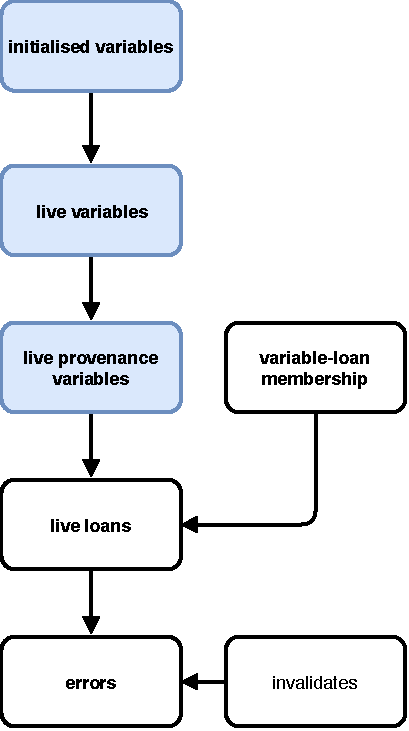
\includegraphics[width=0.4\linewidth]{Graphs/polonius-high-level-overview}
  \caption[Polonius High-Level Overview]{An overview of Polonius high-level
    structure; we compute liveness and members of provenance variables in order
    to find the potentially live loans at every given program point. These
    potential loans are used together with their potential violations to derive
    actual errors. A more precise representation can be found in
    Figure~\ref{fig:polonius-overview}.}
  \label{fig:polonius-high-level-overview}
\end{figure}

We now imagine this typing rule yielding these subtyping constraints for every
assignment in the MIR we are verifying. Polonius only concerns itself with the
attached provenance variables of the types, other parts of the compiler verifies
the rest of the typing judgment. Equipped with this simpler rule, we now have
enough understanding of the formal basis of Polonius to move forward with the
actual implementation.
\chapter{The Borrow Check in the Rust Compiler}\label{cha:borrow-check-compiler}
\epigraph{Get thee to a nunnery, go. Farewell.}%
{Hamlet offering me career advice after my work on this thesis. \textit{Hamlet},
  Act-III, Scene-I}

\begin{figure}[h!]
  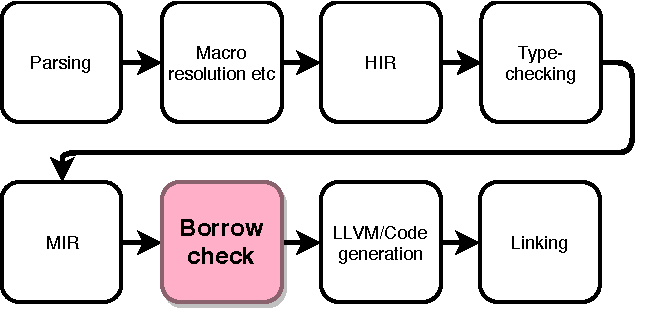
\includegraphics[width=0.9\linewidth]{Graphs/rustc-overview}
  \caption[The Rust Compilation Process]{An overview of the Borrow Check's place
    in the process of compiling Rust code, as described in the Rust Developer's
    Guide~\cite{rustc_developers_guide_nodate}.}
  \label{fig:rustc-overview}
\end{figure}

The logic of the borrow check as described in
Section~\ref{sec:reference-provenance} is calculated at the level of an
intermediate representation of Rust called the Mid-Level Intermediate
Representation (MIR), corresponding to the basic blocks of program control flow.
Rust is lowered to MIR after regular type checking and after a series of earlier
transformations, as seen in Figure~\ref{fig:rustc-overview}. The Polonius
analysis is executed at the function level, checking a function at a time. 

The input data to Polonius is generated in the Rust compiler by analysing this
intermediate representation. This means that we can safely assume to be working
with simple variable-value assignment expressions, of the type \InRust{_1 = _2},
as opposed to complex expressions involving multiple variables on the right-hand
side.

\begin{figure}
\noindent
\begin{minipage}{.5\textwidth}
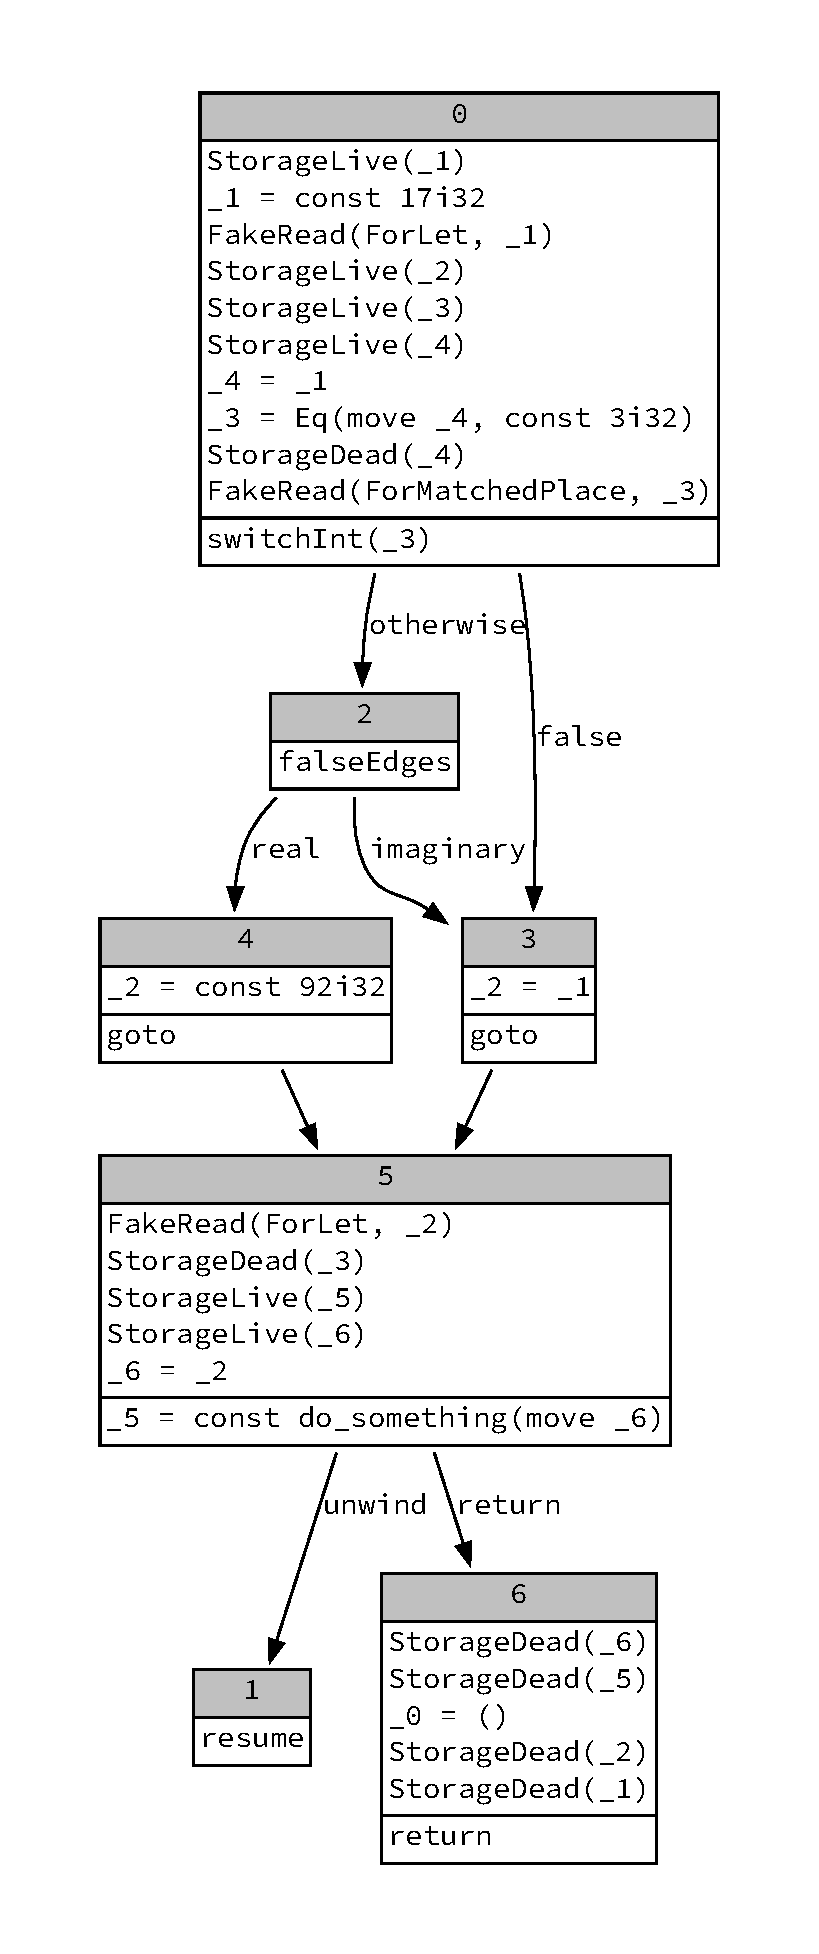
\includegraphics[width=\linewidth]{Graphs/mir-example}
\end{minipage}% This must go next to `\end{minipage}`
\begin{minipage}{.5\textwidth}
  \begin{sourcecode}
  \captionof{listing}{A minimal Rust program featuring branching and a function
    call.}\label{lst:mir-example-input}
\begin{minted}[linenos]{rust}
fn main() {
    let x = 17;
    let z = if x == 3 {
        92
    } else {
        x
    };

    do_something(z);
}
\end{minted}
\end{sourcecode}
\end{minipage}
\caption[MIR of a Small Rust Program With Function Call]{A graph rendering
  (left) of the \InRust{main()} function from a Rust program (right),
  illustrating branching (block 0, corresponding to lines 2--3), and a function
  call (5, corresponding to line 9). Note the \texttt{unwind}~arm of block~5's
  terminator (last line), which will be followed if the function call panics,
  that is if something goes wrong during the call. Blocks~3 and~4 correspond to
  the assignment of the value of the \InRust{if} statement on line 3, assigning
  either \InRust{92} (block~4) or \InRust{x} (block~3) to \InRust{z}. The
  successful return block,~6, contains a number of stack deallocation hints for
  later compilation steps, and sets up the return value of \InRust{main()},
  \InRust{_0} to be the empty tuple (corresponding to \texttt{void} in a
  C~program).}
  \label{fig:mir-example}
\end{figure}

The MIR consists of basic blocks in the traditional compilers sense, each
containing a set of statements and usually ending with a \emph{terminator}, an
expression providing a branching to one or two basic blocks (its
\emph{successors})~\cite{mir_rfc}. A side-to-side comparison between a small
Rust program and its MIR can be seen in Figure~\ref{fig:mir-example}. The
Polonius analysis is performed at the level of these blocks, addressing each
statement of the block in two phases: its start and mid-point. The start of a
block is before the statement has taken effect, and the mid-point is just after.
We use the notation \InRust{Start(bb0[0])} to refer to the starting point of
block 0's first statement, and \InRust{Success(bb5)} to refer to the first
statement of the block following the success branch of basic block~5.

\section{Generating Inputs for Polonius}

The Rust compiler analyses the MIR and emits \textit{facts} that Polonius uses
to derive its conclusions through the Datalog rules described in
Chapter~\ref{cha:implementation}. An overview of the inputs with examples of
when they are used can be seen in Table~\ref{tab:input-facts}, but will be more
closely introduced when they are used. Facts describe relationships between
\textit{atoms}, the objects in the world of Polonius. An overview of the atoms
used in Polonius can be found in Table~\ref{tab:input-atoms}.

{ \renewcommand{\arraystretch}{1.0}
\begin{table}[!htbp]
  \begin{tabular}{@{}l l m{7cm}}
    Atom & Example & Description \\ \hline
    Loan\notmine & \InRust{&x} & An individual borrow expression. \\
    Provenance variable\notmine & \InRust{'a} & The explicit or inferred part of a reference type that contains the set of loans it could have come from.  \\
    Point\notmine & \InRust{Mid(bb1[5])} & A point in the control-flow graph. \\
    Move path & \InRust{x.y.z} & A precise field that can be accessed into a variable; a field in a struct or a projection in a tuple. \\
    Variable & \InRust{x} & A MIR (or Rust) variable. \\
  \end{tabular}
\caption[Polonius Atoms]{The atoms used in Polonius. Variables and move paths
  were introduced as part of this thesis.}
  \label{tab:input-atoms}
\end{table}%
}

{ \renewcommand{\arraystretch}{1.0}
\begin{table}[!htbp]
\begin{tabular}{@{}l l@{} l@{} @{}l@{}}
  Fact & Code Example & Resulting Tuple(s) & Used \\ \hline
  \InDatalog{borrow_region(R, L, P)}\notmine & \InRust{bb0[0]}: \InRust{_1 = &1;}&
                                                                           \InRust{('a, &1, Mid(bb0[0]))} & Bck  \\
  \InDatalog{universal_region(R)}\notmine & \InRust{fn f<'b>(x: &'b str)} & \InRust{('b)} & Bck \\
  \InDatalog{cfg_edge(P, Q)}\notmine &
                               \begin{tabular}[t]{@{}l l@{}}
                                 \InRust{bb0[0]}: & \InRust{_1 = 1;} \\
                                 \InRust{bb0[1]}: & \InRust{_2 = 3;}
                               \end{tabular}
                      &
                        \begin{tabular}[t]{@{}l}
                        \InRust{(Start(bb0[0]), Mid(bb0[0]))},\\
                        \InRust{(Mid(bb0[0]), Start(bb0[1]))},\\
                        \InRust{(Start(bb0[1]), Mid(bb0[1]))}\\
                        \end{tabular}
                        & All \\
  \InDatalog{killed(L, P)}\notmine &
                             \begin{tabular}[t]{@{}l l@{}}
                               \InRust{bb0[0]}: &\InRust{_3 = &_1;} \\
                               \InRust{bb0[1]}: &\InRust{_3 = &_2;}
                             \end{tabular}                                                    
                      &
                        \InRust{(&_1, Mid(bb0[1]))}
                                           & Bck \\
  \InDatalog{outlives(R1, R2, P)}\notmine &
                                    \InRust{bb0[0]}: \InRust{p: &'p i32 = &'x x;}
                                     & \InRust{('x, 'p, Mid(bb0[0]))} & Bck \\
  \InDatalog{invalidates(P, L)}\notmine &
                                  \begin{tabular}[t]{@{}l l@{}}
                                    \InRust{bb0[0]}: & \InRust{_2 = &_1;} \\
                                    \InRust{bb0[1]}: & \InRust{_1 = 3;}
                                  \end{tabular}
                      & \InRust{(Mid(bb0[1]), &_1)} & Bck  \\
  \InDatalog{var_used(V, P)} & \InRust{bb0[0]}: \InRust{x + 1} & \InRust{(x, Mid(bb0[0]))} & Lvs  \\
  \InDatalog{var_defined(V, P)} & \InRust{bb0[0]}: \InRust{x = 7} & \InRust{(x, Mid(bb0[0]))} & Lvs  \\
  \InDatalog{var_drop_used(V, P)} & \InRust{bb0[0]}: \InRust{drop(x)} & \InRust{(x, Mid(bb0[0]))} & Lvs  \\
  \InDatalog{var_uses_region(V, R)} & \InRust{let x: &'x i32;} & \InRust{(x, 'x)} & Lvs  \\
  \InDatalog{var_drops_region(V, R)} &
                                  \begin{tabular}[t]{@{}l@{}}
                                    \InRust{struct Wrap<'p> { p: &'p i32 }} \\
                                    \InRust{impl<'p> Drop for Wrap<'p> {...}} \\
                                    \InRust{let x: Wrap = ...} \\
                                    \InRust{drop(x)}
                                  \end{tabular}
                      & \InRust{(x, 'p)}& Lvs  \\
  \InDatalog{child(M1, M2)} & \InRust{let x = (17, (23, 29));} &
                       \begin{tabular}[t]{@{}l@{}}
                         \InRust{(x.0, x)},\\
                         \InRust{(x.1, x)},\\
                         \InRust{(x.1.0, x.1)},\\
                         \InRust{(x.1.1, x.1)}\\
                        \end{tabular}
                                                           


       & Init  \\
  \InDatalog{path_belongs_to_var(M, V)} & \InRust{let x = (17, (23, 29));} & \InRust{(x, x)} & Init  \\
  \InDatalog{initialized_at(M, P)} & \InRust{bb0[0]}: \InRust{x.0 = 17;} & \InRust{(x.0, Mid(bb0[0]))} & Init  \\
  \InDatalog{moved_out_at(M, P)} & \InRust{bb0[0]}: \InRust{f(move x.0)} & \InRust{(x.0, Start(Success(bb0)))} & Init  \\
  \InDatalog{path_accessed_at(M, P)} & \InRust{bb0[0]}: \InRust{x.val + 7} & \InRust{(x.val, Mid(bb0[0]))} & Init
\end{tabular}
\caption[Input Facts to Polonius]{Polonius input facts, with minimal code
  examples. All facts except \texttt{invalidates}, \texttt{cfg\_edge},
  \texttt{killed}, \texttt{borrow\_region}, \texttt{outlives}, and
  \texttt{universal\_region} were added as part of the work on this thesis.}
  \label{tab:input-facts}
\end{table}%
}

While Polonius is a self-contained package with a single interface, the code
translating compiler-internal data structures into Polonius facts has a much
larger surface area. All the additions to the Rust compiler occurs in the
\texttt{librustc\_mir::borrow\_check::nll}~module, alongside the current borrow
checker (``NLL''). The module hierarchy and the location of emission of the
various facts is shown in Figure~\ref{fig:fact-module-hierarchy}. The reason for
this complex intermingling of modules is that Polonius fact generation
piggy-backs off of previous analysises, notably the \texttt{outlives}
constraints generated by the previous borrow checker during type-checking. In
other words, it is not a full replacement of the current implementation.

\begin{figure}
  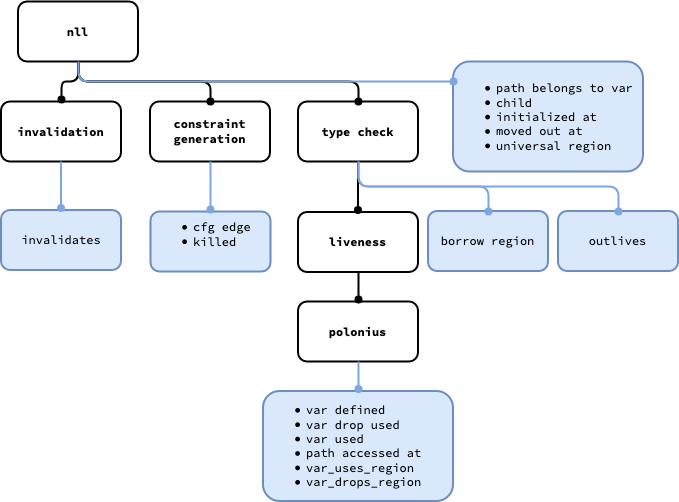
\includegraphics[width=0.9\linewidth]{Graphs/rustc-module-structure}
  \caption[Polonius In Rust's Module Hierarchy]{An illustration of where in the
    module hierarchy of the Rust compiler the various facts are emitted.
    Underscores are replaced with white space for readability. Blue boxes
    represent facts, and black boxes (sub-)modules.}
  \label{fig:fact-module-hierarchy}
\end{figure}

All inputs based on provenance variables (that is, the ones with ``region'' in
their names from the previous terminology); \texttt{path\_belongs\_to\_var},
\texttt{universal\_region}, \texttt{borrow\_region}, \texttt{var\_uses\_region},
and \texttt{outlives}, are all generated using information obtained during
MIR~type-checking. The rest of the inputs are generated either from walking the
MIR directly (\texttt{invalidates}, \texttt{cfg\_edge}, and all the facts
concerning variable uses and drops), or from intermediary indices generated from
the MIR in earlier parts of the compilation process (all facts related to move
paths, which are identified by previous compilation steps). All of this suggests
that the design shown in Figure~\ref{fig:fact-module-hierarchy} should be
refactored to reflect these data dependencies, unifying the generation of most
facts into a common Polonius module higher up in the hierarchy, and leaving only
the ones needing the transient and internal output from the type checker (i.e
provenance variables and their relations to each other and to variables) under
the \texttt{type\_check} submodule. This possible future design is discussed in
more detail in Chapter~\ref{cha:conclusions}.

Returning to one of the examples of the borrowing rules in
Chapter~\ref{cha:borrowing-rules}, we can describe some of the facts that would
be emitted on each line. An annotated example can be seen in
Listing~\ref{lst:polonius-fact-emission}.

\begin{sourcecode}
  \captionof{listing}{A minimal example of a violated loan in Rust and the
    Polonius input facts it would produce during
    compilation.}\label{lst:polonius-fact-emission}
\begin{minted}{rust}
    let mut pt = Point(6, 9); // var_defined(pt)
    let x = &mut pt;  // var_defined(x),
                      // var_used(pt),
                      // borrow_region('1, b0)
                      // outlives('1, 'x)
                      // var_uses_region(x, 'x)
    let y = &mut pt;  // invalidates(b0)
                      // ...

   // we assume var_used(x), var_used(y) is emitted here.
\end{minted}
\end{sourcecode}

The example above is slightly simplified; the translation to MIR would introduce
intermediary variables. However, the core reasoning is the same: the right-hand
side of the assignment is typed with a provenance variable \InRust{'1},
containing only that loan. The assignment to \InRust{x} then sets up a subtyping
relationship with the corresponding \InDatalog{outlives('1, 'x)} fact that
propagates it to \InRust{x}'s provenance variable \InRust{'x}, ensuring it is
considered live when the loan on the next line generates a fact
\InRust{invalidates(b0)}, resulting in the eventual derivation of an
\InRust{error}. Precisely how these errors are derived is the subject of
Chapter~\ref{cha:implementation}.

\chapter{Datafrog, a Datalog Embedded in Rust}\label{cha:datalog}

\epigraph{My liege, and madam, to expostulate\\
  What majesty should be, what duty is,\\
  What day is day, night night, and time is time,\\
  Were nothing but to waste night, day, and time;\\
  Therefore, since brevity is the soul of wit,\\
  And tediousness the limbs and outward flourishes,\\
  I will be brief. Your noble son is mad ...}{Polonius, probably on using
  Datafrog, in \textit{Hamlet}, Act-II, Scene-II}

In this chapter, we will discuss Datalog, the language we use to express
Polonius, and its implementation Datafrog. Datalog is a derivative of the logic
programming language Prolog, with the desirable properties that any program
terminates in polynomial time, and in some variants also with the power to
express all polynomial-time computation~\cite{afrati_datalog_1995}. It describes
fixpoint calculations over logical relations as predicates, described as fixed
input \emph{facts}, computed \emph{relations}, or \emph{rules} describing how to
populate the relations based on facts or other relations. For example, defining
a fact describing that an individual is another individual's child might look
like \InDatalog{child(mary, john).}, while computing the \InDatalog{ancestor}
relation could then use the two rules, reflecting the fact that ancestry is
respectively either direct parenthood or transitive parenthood:
\begin{minted}{rust}
ancestor(Mother, Daughter) :- child(Daughter, Mother).
ancestor(Grandmother, Daughter) :- 
    child(Mother, Grandmother),
    ancestor(Mother, Daughter).
\end{minted}

Datafrog~\cite{datafrog} is a minimalist Datalog implementation embedded in
Rust, providing an implementation of a worst-case optimal join algorithm as
described in~\cite{ngo_worst-case_2012}. The fact that Datafrog is embedded in
Rust (an EDSL) means that standard Rust language abstractions are used to
describe the computation. Static facts are described as \InRust{Relation}s,
while dynamic \InRust{Variable}s are used to capture the results of
computations, both of which are essentially sets of tuples, in our case tuples
of integers. Rules are described using a join with either a \InRust{Variable} or
a \InRust{Relation}, with an optimised join method used for joins with only one
variable, but multiple relations. Only single-step joins on the first tuple
element are possible, which means that more complex rules must be written with
intermediary variables, and manual indices created whenever a relation must be
joined on a variable which is not the first in the tuple. An example of the
\InDatalog{ancestor} relation in Datafrog can be seen in
Listing~\ref{lst:datafrog:ancestor}.

\begin{sourcecode}
  \captionof{listing}[\InDatalog{ancestor(X, Y)} in
  Datafrog.]{\InDatalog{ancestor(X, Y)} in Datafrog. Note the \InRust{map()}
    invocation, which reverses the tuples of the input \InRust{Vec} to fit the
    reversed target order. This example is used in work-in-progress Polonius
    code used to derive children of move paths, which is otherwise left outside
    of the scope of this thesis.}\label{lst:datafrog:ancestor}
\begin{minted}{rust}
let ancestor = iteration.variable::<(T::Path, T::Path)>("ancestor");

// ...

// ancestor(Mother, Daughter) :- child(Daughter, Mother).
ancestor.insert(
    child
        .iter()
        .map(|&(child_path, parent_path)| (parent_path, child_path))
        .collect(),
);

// ancestor(Grandmother, Daughter) :-
ancestor.from_join(
    &ancestor, // ancestor(Mother, Daughter),
    &child,    // child(Mother, Grandmother).
    // select the appropriate part of the match:
    |&_mother, &daughter, &grandmother| (grandmother, daughter),
);
\end{minted}
\end{sourcecode}

\begin{sourcecode}
  \captionof{listing}{The implementation of \InDatalog{var_use_live(V, P)} in
    Datafrog.}\label{lst:datafrog:var-live}
\begin{minted}{rust}
var_use_live_var.from_leapjoin(
    &var_use_live_var,
    (
        var_defined_rel.extend_anti(|&(v, _q)| v),
        cfg_edge_reverse_rel.extend_with(|&(_v, q)| q),
    ),
    |&(v, _q), &p| (v, p),
);
\end{minted}
\end{sourcecode}

Moving on with a more complex example, the Datafrog code for
\InDatalog{var_use_live(V, P)} of Listing~\ref{lst:var-live} becomes the code in
Listing~\ref{lst:datafrog:var-live}, and the corresponding join used for the
first half of \InDatalog{region_live_at(R, P)} of
Listing~\ref{lst:region-live-at} can be seen in
Listing~\ref{lst:datafrog:region-live-at}.

\begin{sourcecode}
  \captionof{listing}{The first half of the implementation of
    \InDatalog{region_live_at(R, P)} in
    Datafrog.}\label{lst:datafrog:region-live-at}
\begin{minted}{rust}
region_live_at_var.from_join(
    &var_drop_live_var, 
    &var_drops_region_rel, 
    |_v, &p, &r| {
        ((r, p), ())
    });
\end{minted}
\end{sourcecode}

Joins in Datafrog are done using one of two methods on the variable that is to
be populated (e.g. in Listing~\ref{lst:datafrog:region-live-at}
\InRust{region_live_at_var}), a variable with tuples of the format \InRust{(Key,
  Val1)}. The first method, \InRust{from_join}, performs simple joins from
variables or relations into the (possibly different) target variable. Its
arguments, in order, are a \InRust{Variable} of type \InRust{(Key, Val2)}, and
either a second \InRust{Variable} or a \InRust{Relation} of type \InRust{(Key,
  Val3)}. The third and final argument is a combination function that takes each
result of joining the two non-target arguments, a tuple of type \InRust{(Key,
  Val2, Val3)}, and returns a tuple of format \InRust{Key, Val1} to be inserted
into the target variable.

In the example of Listing~\label{lst:datafrog:region-live-at}, the target
variable~\InRust{region_live_at_var} is populated by joining the
\InRust{Variable} \InRust{var_drop_live_var} to the \InRust{Relation}
\InRust{var_drops_region_rel}. Here, the combination function ignores the
variable, returning only the resulting provenance variable and CFG point. The
final result is stored in the first half of \InRust{region_live_at} with the
empty tuple as the second half. This is a work-around to enable joins with two
two-tuples.

For more complex joins where a single variable participates in the join and all
other arguments are static \InRust{Relation}s (such as is the case with the
variable~\InRust{var_use_live_var} of Listing~\ref{lst:datafrog:var-live}), there is
\InRust{from_leapjoin}. In this case, the input is the sole dynamic source
variable, a tuple of ``leapers'', and a combining function like the one in
\InRust{from_join}, but with the signature like the one above, mapping a matched
tuple from the join to the target of the join.

A leaper is created from a \InRust{Relation} of type \InRust{(Key, Value)} by
either applying the method \InRust{extend_with} or \InRust{extend_anti} for a
join or an anti-join respectively. Both of these functions then take a function
mapping tuples from the \InRust{Variable} to \InRust{Key}s in the
\InRust{Relation} being (anti-)joined. In the case of \InRust{extend_anti}, any
tuples matching \InRust{Key} are discarded.

In Listing~\ref{lst:datafrog:var-live}, we can see a leapjoin populating
\InRust{var_use_live_var} with tuples produced by joining the \InRust{Relation}s
representing \InRust{var_defined_rel} and the reversed CFG.

\section{Why Datalog?}\label{sec:why-datalog}

Datalog has a long history of use for static analysis, with a notable recent
example being the Souffl{\'e} system, which synthesises performant C++ code from
the Datalog specifications to show promising performance for analysis of large
programs comparable to hand-crafted implementations in
C++~\cite{scholz_fast_2016}. This approach is similar to how Datafrog embeds a
minimal solver as a Rust library. Souffl{\'e} in particular was an inspiration
for Polonius, and with the current ongoing work on translating Souffl{\'e}-style
Datalog into the more cumbersome Datafrog EDSL format Polonius can almost be
said to converge into a specialised ``Souffl{\'e} for Rust''.\footnote{The
  experimental code to synthesise Datafrog rules can be found on GitHub in the
  separate repository \url{https://github.com/lqd/datapond}.}

Another inspiration was the \textsc{Doop}
framework~\cite{smaragdakis_using_2010}, developed by
\citeauthor*{smaragdakis_using_2010} for a proprietary Datalog engine and later
ported to Souffl{\'e}~\cite{doop-porting}. \textsc{Doop} specifically performs a
may-point-to-analysis (much like Polonius), using explicit tuple storage (also
like Polonius), as opposed to other common representations like Binary Decision
Diagrams (BDDs). Much like Polonius, the authors of Doop sought a framework that
would let them specify their analysis clearly in a high-level language. In fact,
Datalog has been so successful for may-point-to-analysis that a 2016~paper
developing a lattice-based declarative analysis for the same purpose described
it as ``the killer application'' of
Datalog~\cite{Madsen:2016:DFD:2980983.2908096}, a career that took off
around~\citeyear{Benton:2007:ISD:1273920.1273923} with the work of
\citeauthor{Benton:2007:ISD:1273920.1273923}, who demonstrated the
\textsc{Dimple} framework for static analysis of
Java~\cite{Benton:2007:ISD:1273920.1273923}. This was despite a case study
showing already in~\citeyear{Dawson:1996:PPA:231379.231399} that logic
programming (in that case Prolog) would constitute a good trade-off between
performance of the analysis and efficiency of
development~\cite{Dawson:1996:PPA:231379.231399}.

However, and as mentioned in Section~\ref{sec:contributions}, Polonius is to our
knowledge the first attempt at using Datalog for pointer analysis (or any other
kind of static analysis for that matter) in a production compiler. All the
previous analyses and frameworks have been predominantly analysis of Java,
either in the form of source code or byte code, by programs outside of the Java
compiler.


\chapter{Implementing Polonius}\label{cha:implementation}

\epigraph{Why, then, 'tis none to you, for there is nothing either good or bad,
  but thinking makes it so}%
{\textit{Hamlet}, Act-II, Scene-II}

In this chapter, we will describe the current implementation of Polonius in
Datalog (forgetting the horrors of Datafrog in Section~\ref{sec:datalog}). We
will start by discussing how information (``facts'') extracted from the
user-supplied program via the MIR (introduced in
Section~\ref{sec:rust-specificts}) flows through the Polonius analysis to
determine if and where the conditions of a loan are violated. We will then go
into detail about the actual Datalog rules of Polonius in
Section~\ref{sec:borr-check-datal}, discuss how the input facts are generated in
the Rust compiler (Section~\ref{lst:polonius-fact-emission}), and finish up by
discussing what is missing in Polonius in order to perform a full analysis
(Section~\ref{sec:missing-features}).

An overview of Polonius can be seen in Figure~\ref{fig:polonius-overview}:
initialisation is calculated in order to calculate drop-liveness, which together
with regular use-liveness is used to determine the actual liveness of variables.
The liveness of variables is then used to determine the liveness of provenance
variables in their types, and is used throughout the calculations. Subset
relations between provenance variables are used to determine the set membership
of loans, and those are then combined with the liveness information in order to
determine which loans are live at which point of the program flow. Errors,
finally, are generated whenever a potentially violating operation happens to a
live loan (an observed tree falls in the woods, thus making a sound).

\begin{figure}
  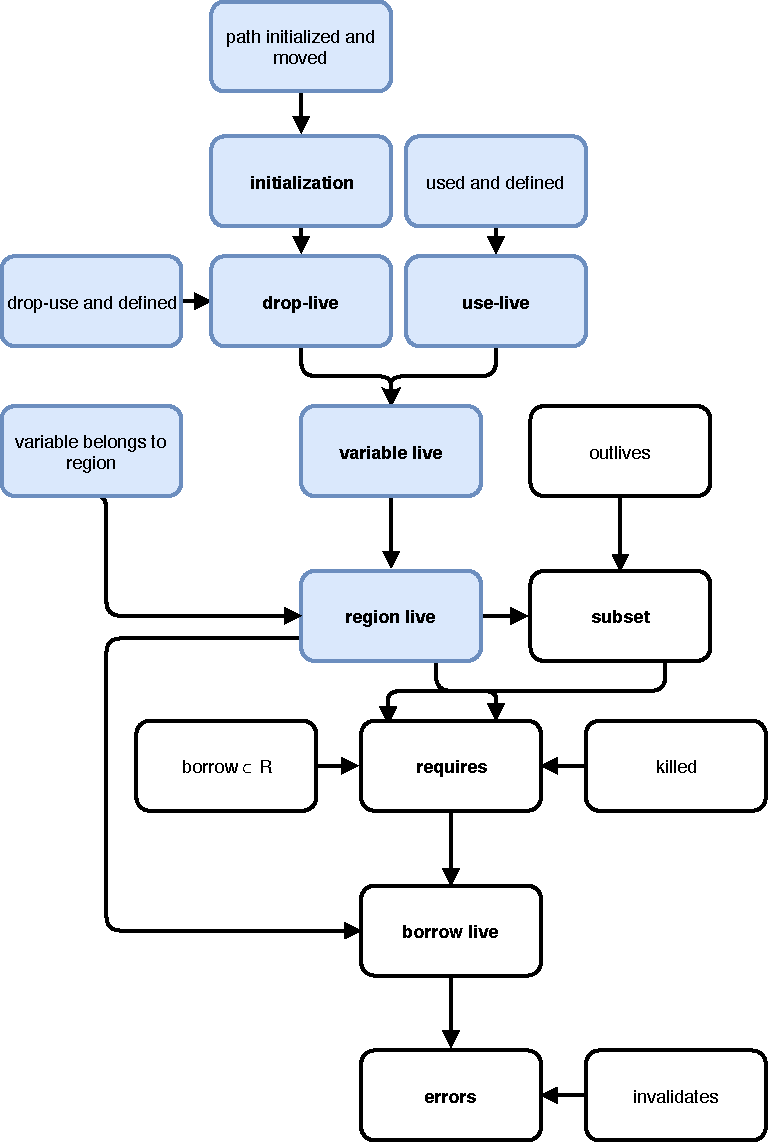
\includegraphics[width=0.9\linewidth]{Graphs/polonius-overview}
  \caption[Flowchart of the Polonius Inputs and Outputs]{An overview of how the
    inputs and intermediate steps of Polonius combine into the final output.
    Blue boxes represent facts and relations implemented during the work on this
    thesis. Relations are shown using boldface, and facts in regular font. The
    historical term ``region'' is used here instead of provenance variables to
    match the convention used in the actual code.}
  \label{fig:polonius-overview}
\end{figure}

\section{What Is Being Borrowed and Moved?}\label{sec:paths}

The borrow check specifically tracks memory at the resolution of \textit{paths},
that is paths to concrete memory. Examples of paths is \InRust{x} (a variable on
the stack), \InRust{x.f} (a field of a \InRust{struct}), \InRust{*x.f} (a field
accessed through a reference), or \InRust{(*x.f)[_]} (an index of an array
stored in a \InRust{struct} and accessed through a reference). However, an array
counts as one path, ignoring its indices. Paths constitute trees, (or perhaps
rather Russian nesting dolls) such as in the example of \InRust{x.f}, where
\InRust{x.f} lies under \InRust{x}. We say that each path preceding (and
including) a given path are its \textit{prefixes}. The topmost path, the
variable name itself, we call a \textit{root path}. Finally, we say that paths
\textit{overlap} if one of them is a prefix of the other. Intuitively, this mean
that they involve the same region in memory.


The fact that the borrow check is performed on paths means that the following
code, for example, is sound, as the paths and therefore also the loans do not
overlap:
\begin{minted}{rust}
struct Point(u32, u32);

let mut pt: Point = Point(6, 9);
let x = &mut pt.0;
let y = &mut pt.1;
// no error; our loans do not overlap!
\end{minted}

\section{Liveness, as Experienced by Polonius}\label{sec:liveness}

A summary of the facts, intermediate relations, and outputs of Polonius'
liveness computations can be found in Table~\ref{tab:liveness-facts-recap}.

{ \renewcommand{\arraystretch}{1.0}
\begin{table}[!htbp]
  \begin{tabular}{@{}l l m{5.5cm}}
    Atom/Fact & Type & Description \\ \hline
    Provenance\notmine & Atom & The explicit or inferred part of a reference type that contains the set of loans it could have come from.  \\
    Point\notmine & Atom & A point in the control-flow graph. \\
    Variable & Atom & A MIR (or Rust) variable. \\
    \InDatalog{cfg_edge(P, Q)}\notmine & Fact & A transition in the CFG. \\
    \InDatalog{var_used(Var, Point)} & Fact & A regular variable use happens here.\\
    \InDatalog{var_defined(Var, Point)} & Fact & A variable is assigned here.\\
    \InDatalog{var_uses_region(Var, Provenance)} & Fact & Connects provenance variables from types to their variables.\\
    \InDatalog{var_drops_region(Var, Provenance)} & Fact & Deallocating this variable indirectly uses this provenance variable. \\
    \InDatalog{var_initialized_on_entry(V, Point)} & Fact & This variable is initialised on entry to this CFG node. \\
    \InDatalog{var_drop_live(Var, Point)} & Intermediate & This variable is used in a drop. \\
    \InDatalog{var_use_live(Var, Point)} & Intermediate & This variable is used in an expression. \\
    \InDatalog{region_live_at(Provenance, Point)} & Output & This provenance variable is live at this point, and the conditions of its loan must be accepted. \\
  \end{tabular}
\caption[Liveness Dramatis Personae]{Liveness Dramatis Personae.}
  \label{tab:liveness-facts-recap}
\end{table}%
}

\begin{figure}
  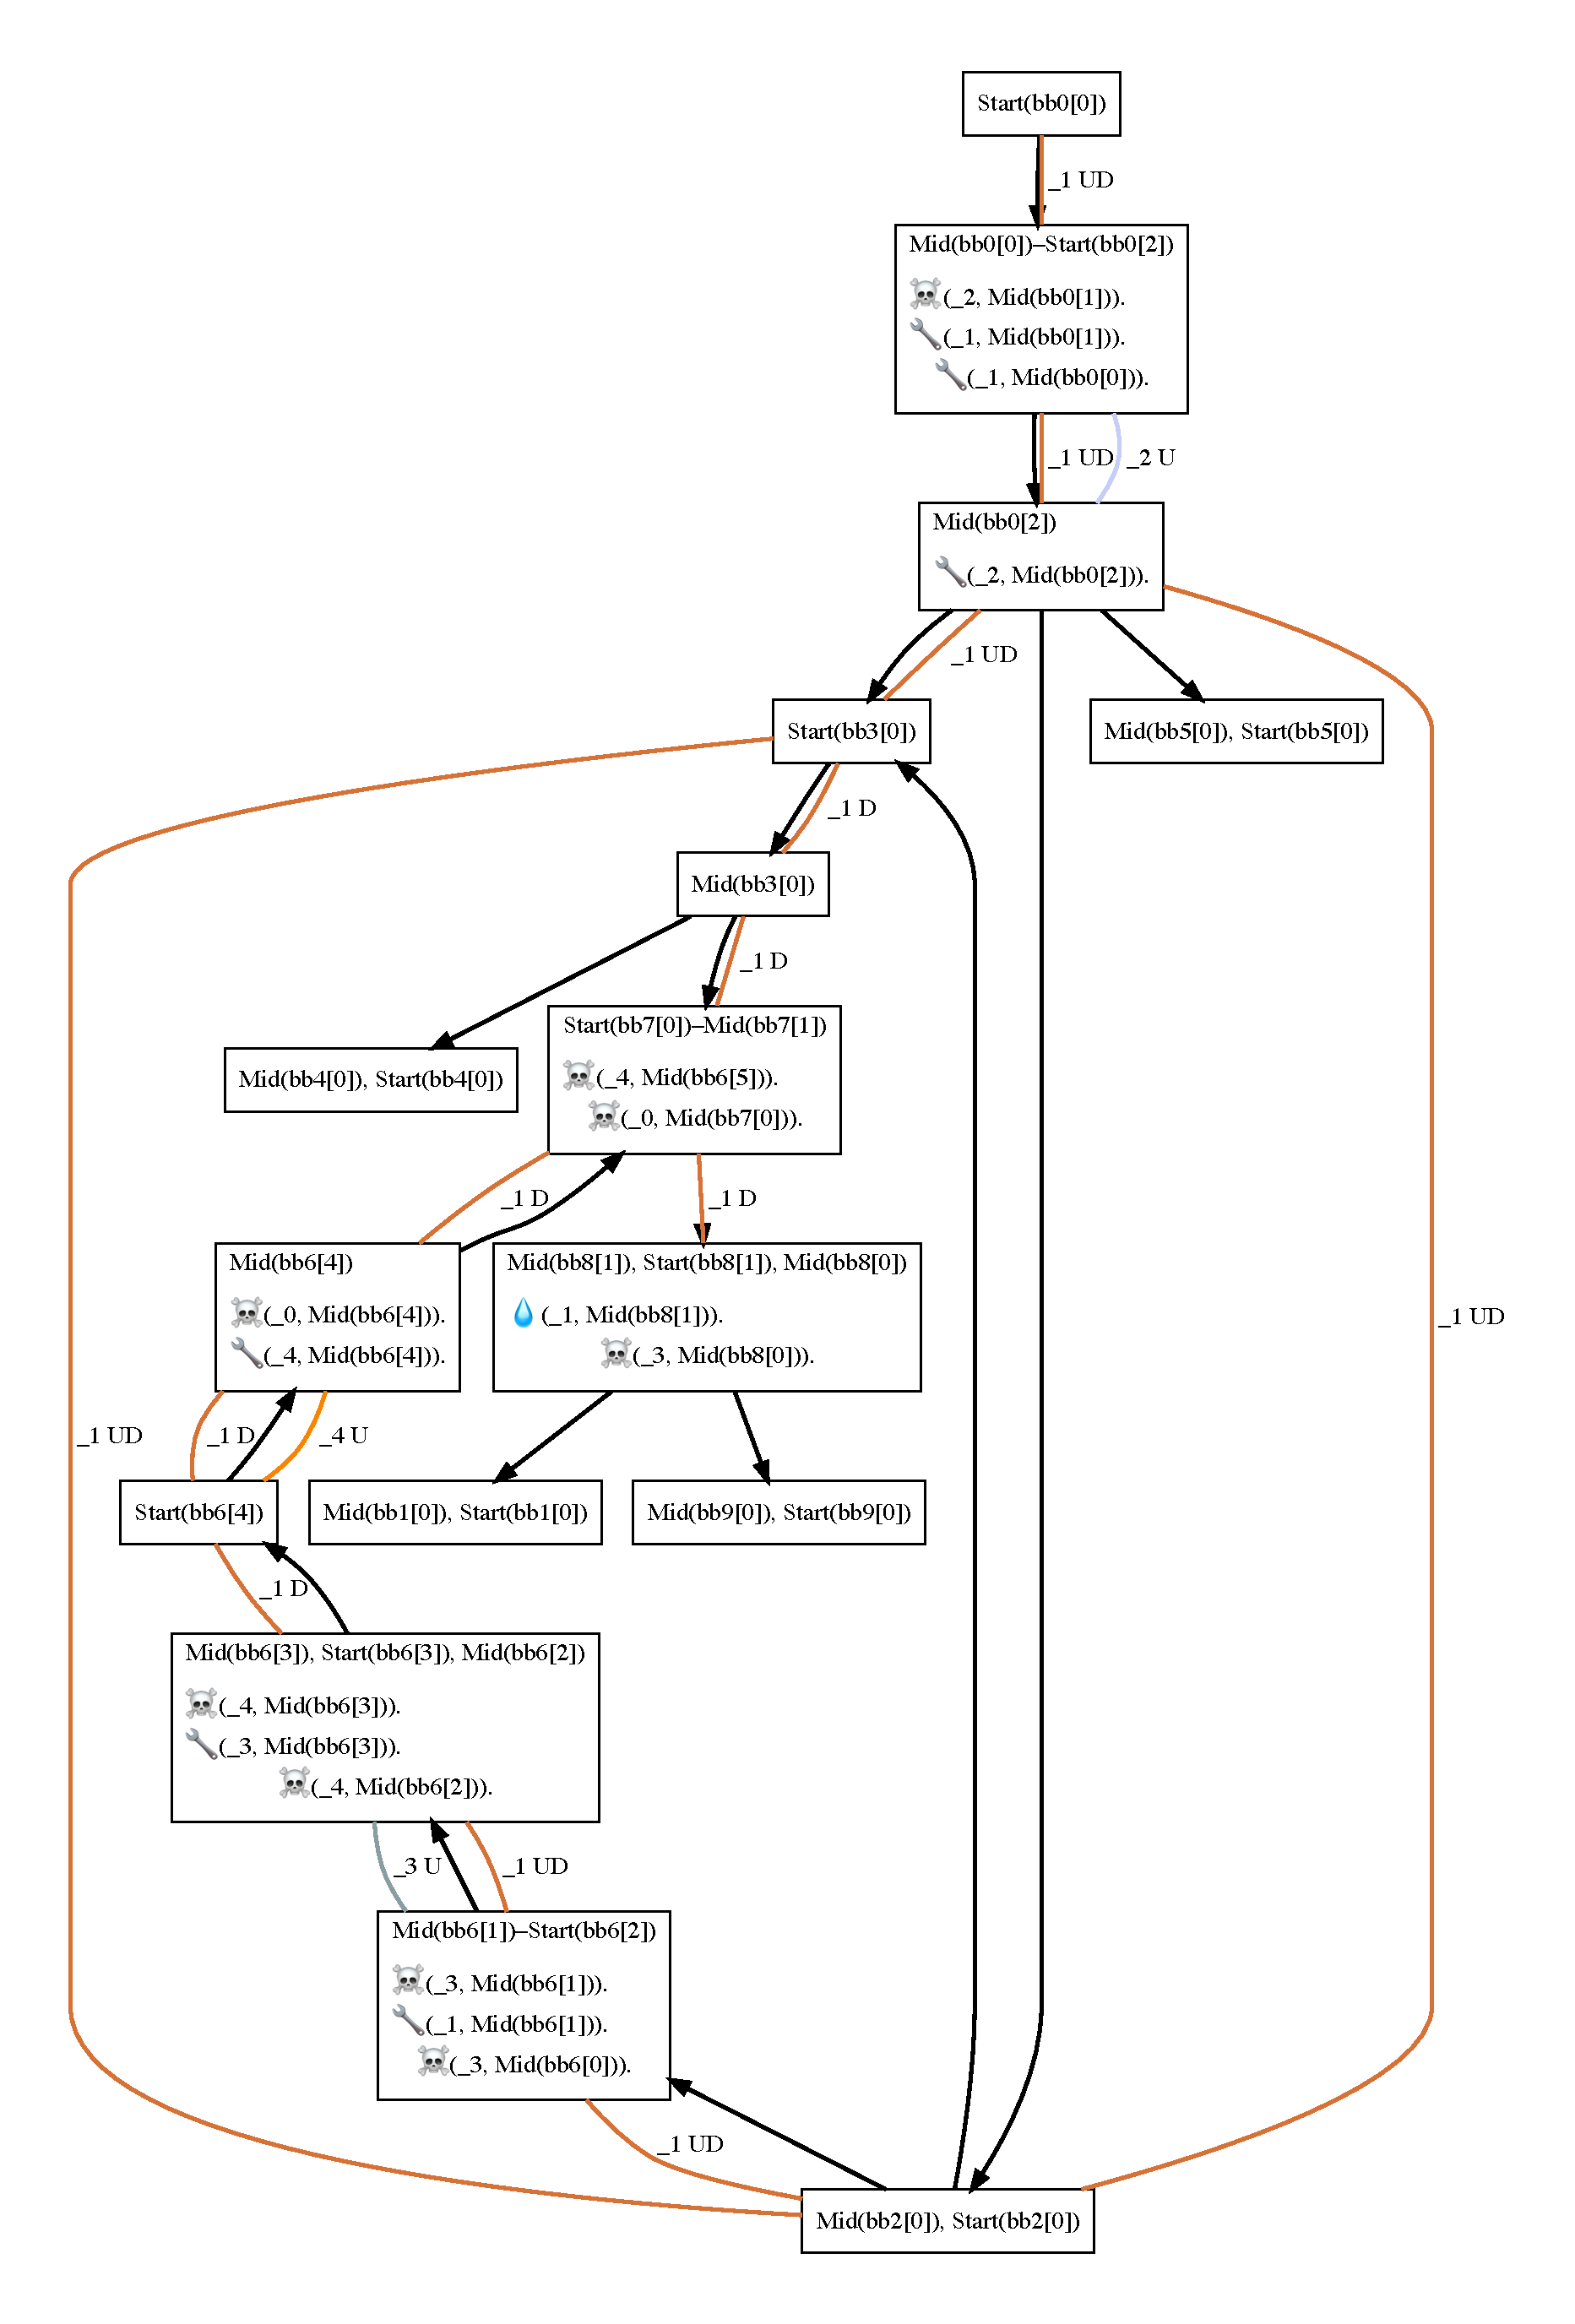
\includegraphics[width=0.9\linewidth]{Graphs/liveness.pdf}
  \caption[MIR Fragment with Inputs and Outputs of the Liveness Analysis]{A
    graph representation of the the variable liveness calculation results, with
    relevant Polonius facts as they occur (a droplet symbolising
    \InDatalog{var_drop_used}, a wrench \InDatalog{var_used}, and a skull and
    crossbones symbolising \InDatalog{var_defined}). Variables are named by
    prefixing underscores, and edges annotated with the propagated live variable
    and its liveness type(s) (\textbf{D}rop or \textbf{U}se).}
  \label{fig:liveness-graph}
\end{figure}

The basic liveness of a variable (Listing~\ref{lst:var-live}) is computed
similarly to variable initialisation, except with variable uses instead of
initialisations, assignments instead of uses, and backwards across the CFG.
Specifically, the rule is as follows: if a variable~$v$ is live in some
point~$q$ and~$q$ is reachable from $p$ in the control-flow graph, then~$v$ is
live in~$p$ too unless it was overwritten. Like initialisation, it is also
imprecise with respect to branchings, as there is no way to know statically
which branch is taken. We refer to this type of liveness as
\textit{use-liveness}, owing to the fact that the liveness comes from variable
use.

\begin{figure}
\begin{sourcecode}
\begin{minted}{prolog}
var_use_live(V, P) :- var_used(V, P).

var_use_live(V, P) :-
    var_use_live(V, Q),
    cfg_edge(P, Q),
    !var_defined(V, P).
\end{minted}
\end{sourcecode}

{ \renewcommand{\arraystretch}{1.5}
    \begin{tabular}{@{}l l}
      Positive & \begin{tabular}[t]{@{}l  l@{}}
                   Input & Conclusion \\ \hline
                   \begin{tabular}[t]{@{}l}
                     \InRust{var_used(x, Start(bb0[1]))}\\
                     \InRust{cfg_edge(Mid(bb0[0]), Start(bb0[1]))}
                   \end{tabular} &%
                                   
                   \begin{tabular}[t]{@{}l}
                     \InRust{var_use_live(x, Mid(bb0[0]))} \\
                     \InRust{var_use_live(x, Start(bb0[1]))}
                   \end{tabular}
                       
                 \end{tabular}\\
      Negative & \begin{tabular}[t]{@{}l  l@{}}
                   Input & Conclusion \\ \hline
                   \begin{tabular}[t]{@{}l}
                     \InRust{var_use_live(x, Start(bb0[1]))}\\
                     \InRust{var_defined(x, Mid(bb0[0]))}\\
                     \InRust{cfg_edge(Mid(bb0[0]), Start(bb0[1]))}
                   \end{tabular} &%
                                   (nothing)
                 \end{tabular}\\
    \end{tabular}    
  }

  \caption[Rules for Calculating Use-Liveness]{The rules for calculating
    use-liveness: a variable is use-live if it was used at a point $P$, or if it
    was live in $Q$, there is a transition $P\rightarrow{}Q$, and it was not
    defined (killed) in $P$.}\label{fig:var-use-live}

\end{figure}

\subsection{Deallocation As a Special Case of Variable Use}
\label{sec:deall-as-spec}
When Rust's variables go out of scope, they are implicitly deallocated, or
dropped in Rust parlance. Explicit deallocation is also possible by calling the
function \InRust{drop()}, which takes ownership of a variable (that is,
deinitialises it) and performs deallocation, or, for complex objects, calls the
\InRust{drop()} method.

Rust provides a default deallocator for data structures, which can be
overridden. This has repercussions on liveness calculations. While the default
deallocator for an object never accesses its fields, and therefore does not make
them live, a custom deallocator might access any of them in arbitrary ways. This
of includes references stored in the struct, whose provenance variables must be
considered live. Intuitively, this follows from the fact that the deallocator
may use the references in the \InRust{struct}, and that the conditions of their
loans must therefore be respected, and we say that the variable holding the
struct is \textit{drop-live}. An example can be found in
Figure~\ref{fig:drop-liveness}.


\begin{figure}
\noindent
\begin{minipage}{.5\textwidth}
  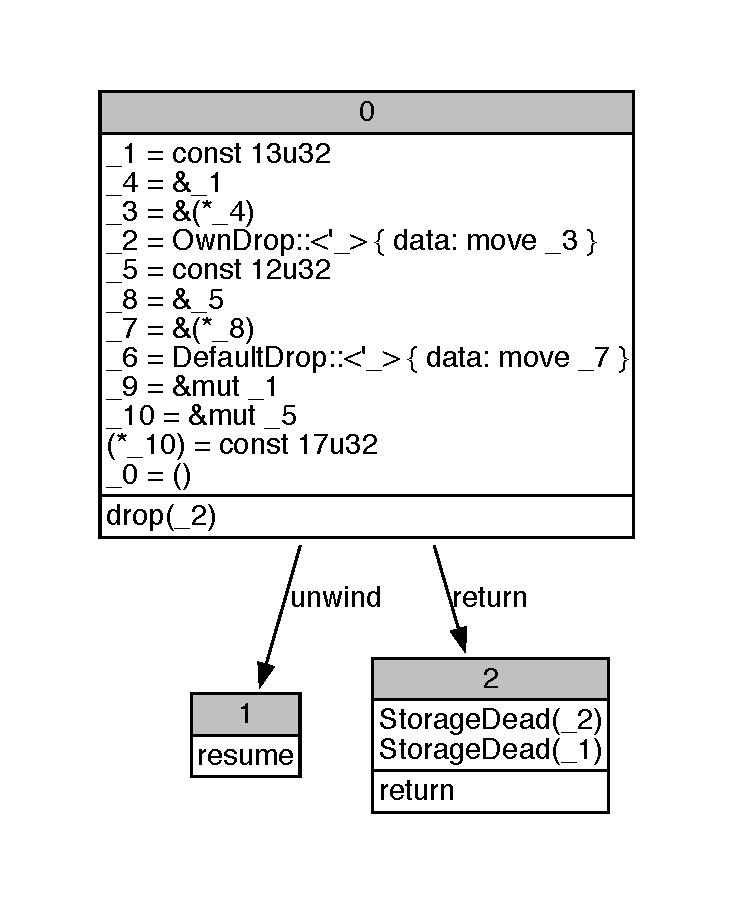
\includegraphics[width=\linewidth]{Graphs/drop-main-mir}
\end{minipage}% This must go next to `\end{minipage}`
\begin{minipage}{.5\textwidth}
\begin{sourcecode}
  \captionof{listing}{The custom deallocator for \InRust{OwnDrop} enforces the
    loan giving the reference \InRust{data} until the struct is deallocated, but
    the loan in \InRust{DefaultDrop} is effectively dead as soon as it has no
    direct uses in the code and thus can be violated.}\label{lst:drop-liveness}
\begin{minted}{rust}
struct OwnDrop<'a> {
    data: &'a u32,
}

struct DefaultDrop<'a> {
    data: &'a u32,
}

impl<'a> Drop for OwnDrop<'a> {
    fn drop(&mut self) {
        // might access self.data
    }
}

fn main() {
    let mut x = 13;
    let a = OwnDrop { data: &x };

    let mut y = 12;
    let b = DefaultDrop { data: &y };
    
    let mutrefa = &mut x;
    // ERROR: the loan of x must be respected...
    
    // ...but the loan of y need not be!
    let mutref = &mut y;
    *mutref = 17;
    
    // all variables are implicitly dropped here
}
\end{minted}
\end{sourcecode}
\end{minipage}
\caption[MIR of a Program Utilising a Custom Deallocator]{A graph rendering of
  the MIR produced from the \InRust{main()} function of the code to the right,
  illustrating a call to the custom deallocator of~\InRust{_2} that would cause
  it to be drop-live during the block. Take special note of the lack of calls to
  \InRust{drop(_6)}; as \InRust{DefaultDrop}, the \InRust{struct} stored in
  \InRust{_6}, uses the default deallocator and contains only a reference,
  deallocating it is a no-op. Some irrelevant details, such as hints about stack
  allocations and deallocations of intermediate variables, have been pruned.}
  \label{fig:drop-liveness}
\end{figure}

Following the MIR translation of Listing~\ref{lst:drop-liveness} in
Figure~\ref{fig:drop-liveness}, we see across the re-borrows used to move the
created references into the \InRust{struct}s that the function's single block
terminates in a call to \InRust{drop()} that would invoke the custom
deallocator. Here, the deallocator for \InRust{b}, our instance of
\InRust{DefaultDrop}, is never even called at all, as its sole element, a
reference, requires no deallocation.

Drop-liveness is calculated in a similar fashion to use-liveness, with the
exception that a moved variable is never dropped, as it is now owned (and
therefore deallocated) by the context it was moved to. This is the reason for
the computation of variables that might be initialised in
Section~\ref{sec:move-analysis}. The rules can be found in
Listing~\ref{lst:drop-live}.

Note the use of the first rule, which is not transitive, to shift the point of
the initialisation from the input's mid-point index (which is where a
(de)initialisation would take effect) to the statement's starting-point. This is
because a drop-use would only happen if the \InRust{x} was initialised on
\textit{entry} to the instruction \InRust{drop(x)}.

\begin{sourcecode}
  \captionof{listing}{The rules for calculating drop-liveness: the rules are
    similar to those for to use-liveness (Listing~\ref{lst:var-live}), but
    propagation of liveness only happens if the variable being dropped may be
    initialised. Note that the rule for calculating initialisation on entry is
    not transitive!}\label{lst:use-live}
\begin{minted}{prolog}
var_maybe_initialized_on_entry(V, Q) :-
    var_maybe_initialized_on_exit(V, P),
    cfg_edge(P, Q).

var_drop_live(V, P) :-
    var_drop_used(V, P),
    var_maybe_initialzed_on_entry(V, P).

var_drop_live(V, P) :-
    var_drop_live(V, Q),
    cfg_edge(P, Q),
    !var_defined(V, P)
    var_maybe_initialized_on_exit(V, P).
\end{minted}
\end{sourcecode}

\subsection{Variable Liveness to Provenance Variable Liveness}\label{sec:region-live-at}

The two kinds of liveness are then used to calculate the reference liveness
relation (Listing~\ref{lst:region-live-at}), which serves as input for the rest
of the borrow checker. A given provenance variable~$R$ is live at some point~$p$
if it is in the type of a use-live variable~$v$, or if it is associated to a
drop-live variable. While the connection between use-live variables and their
provenances is direct, the connection between a use-live variable and its
provenance variable(s) is \textit{indirect}; any reference stored inside the
drop-live \InRust{struct} in~$v$ is live at~$p$ if~$v$ is drop-live there. An
example of this can be seen in Table~\ref{tab:liveness-example}.

\begin{sourcecode}
  \captionof{listing}{A provenance variable is live if it either belongs to a
    use-live variable, or if it might be dereferenced during the deallocation of
    a drop-live variable.}\label{lst:region-live-at}
\begin{minted}{prolog}
region_live_at(R, P) :-
    var_drop_live(V, P),
    var_drops_region(V, R).
        
region_live_at(R, P) :-
        var_use_live(V, P),
        var_uses_region(V, R).
\end{minted}
\end{sourcecode}

{ \renewcommand{\arraystretch}{1.0}
\begin{table}[!htbp]
\begin{tabular}{@{}l l l l}
  Statement & Use-live & Drop-live & Provenance(s) live \\ \hline
  \InRust{let mut x = 13;} \\
  \InRust{let own = OwnDrop { data: &'x1 x };} & \InRust{x} & &  \\
  \InRust{let bad_ref = &'x2 mut x;} & \InRust{x} & \InRust{own} & \InRust{'x1}  \\
  \InRust{uses_var(bad_ref);} & \InRust{bad_ref} & \InRust{own} & \InRust{'x2, 'x1}  \\
  \InRust{// drop(own) implicit} & & \InRust{own} & \InRust{'x2} \\
\end{tabular}
\caption[Liveness Example]{An example of a drop-live \InRust{struct} causing an
  inner provenance variable to be live. This program would generate an error, as
  we have two overlapping loans of the same path, where one is mutable.}
  \label{tab:liveness-example}
\end{table}%
 }

\section{Move Analysis}\label{sec:move-analysis}

{ \renewcommand{\arraystretch}{1.0}
\begin{table}[!htbp]
  \begin{tabular}{@{}l l m{5.5cm}}
    Atom/Fact & Type & Description \\ \hline
    Provenance\notmine & A & The explicit or inferred part of a reference type that contains the set of loans it could have come from.  \\
    Point\notmine & A & A point in the control-flow graph. \\
    Variable & A & A MIR (or Rust) variable. \\
    Path & A & A move path. \\
    \InDatalog{cfg_edge(P, Q)}\notmine & F & A transition in the CFG. \\
    \InDatalog{child(Path2, Path1)} & F & \InDatalog{Path1} is a prefix of-, and not equal to \InDatalog{Path2}  \\
    \InDatalog{initialized_at(Path, P)} & F, I & This path was given a value here. \\
    \InDatalog{path_belongs_to_var(Path, V)} & F & This path is the root path of variable $V$. \\
    \InDatalog{path_accessed_at(Path, Point)} & F, I & This move path is used in an expression here.\\
    \InDatalog{moved_out_at(Path, P)} & F, I & This path was moved from this scope in an expression here. \\
    \InDatalog{ancestor(Above, Below)} & I & \InDatalog{Above} is a prefix of \InDatalog{Below}.\\
    \InDatalog{path_maybe_init___exit(Path, Point)} & I & \InDatalog{Path} is initialized without subsequent deinitialisation on one or more branches reaching this CFG node (lowest upper bound on set membership).\\
    \InDatalog{path_definitely_init___(Path, Point)} & I &  \InDatalog{Path} is initialised on all branches reaching \InDatalog{Point} (greatest lower bound on membership). \\
    \InDatalog{path_maybe_mov___(Path, Point)} & I & \InDatalog{Path} has been moved without subsequent reinitialisation on at least one branch reaching this CFG node. \\
    \InDatalog{var_maybe_init___(Var, Point)} & O & This variable is initialised along at least one branch reaching this node at the time of its exit. \\
    \InDatalog{move_error(Path, Point)} & O & Error: \InDatalog{Path} is accessed here, but may have been moved, or was never initialised. \\
  \end{tabular}
\caption{Move Analysis Dramatis Personae}
  \label{tab:move-facts-recap}
\end{table}%
}

The idea behind the move analysis is a fairly straightforward transitive closure
computation. Initialisation (\InDatalog{path_initialized_lub_exit}) propagates
forwards from an assignment (\InDatalog{initialized_at}) across the CFG
(\InDatalog{cfg_edge}) until the path is moved (\InDatalog{moved_out_at}). We
also transitively follow the move path tree downwards on each event, so that a
use of \InRust{x} would also use \InRust{x.f}, for example. This transitive
expansion of facts happens in a pre-computation described in
Section~\ref{sec:move:fixpoints}. Finally, we trace root paths (and therefore
also their transitive children) back to their variables through
\InDatalog{path_belongs_to_var}. A summary of the inputs, outputs, and
intermediary relationships involved in the computation can be found in
Table~\ref{tab:move-facts-recap}.

However, Rust programs like all Turing-complete programs, are not deterministic.
Therefore initialisation tracking is necessarily imprecise upon branching; if
one branch in the CFG has \InDatalog{Path} initialised and one does not, we must
decide on whether to over-estimate (assume \InDatalog{Path} is initialised), or
under-estimate (assume \InDatalog{Path} is deinitialised) after the branches
join. As it turns out, the move analysis does both. When we want to determine if
a variable might be involved in a deallocation for the purposes of later
figuring out live references in Section~\ref{sec:deall-as-spec}, we
over-estimate (Section~\ref{sec:var-maybe-initialised}). When we want to figure
out if it is safe to access a variable or if we should generate a move error, we
under-estimate (Section~\ref{sec:move-errors}).

\subsection{Figuring Out The Move Tree}\label{sec:move:fixpoints}

The analysis begins with a pre-computation step that expands the path-related
facts so that an initialisation of a prefix also initialises its children,
grandchildren, etc. The Datalog for this can be found in
Listings~\ref{lst:ancestor} and~\ref{lst:transitive-moves}. The transitive
expansion happens for all the path-related facts: \InDatalog{initialized_at},
\InDatalog{accessed_at}, \InDatalog{moved_out_at}, and \InDatalog{child} (which
becomes \InDatalog{ancestor}). The names are re-used in later steps to reflect
the fact that we see this as a pre-computation step expanding compressed facts
from Rust.

\begin{sourcecode}
  \captionof{listing}{Calculating the move path tree; a path is the
    \InDatalog{ancestor} of all its children and their children
    transitively.}\label{lst:ancestor}
\begin{minted}{prolog}
ancestor(Mother, Daughter) :- child(Daughter, Mother).

ancestor(Grandmother, Daughter) :-
    ancestor(Mother, Daughter),
    child(Mother, Grandmother).
\end{minted}
\end{sourcecode}

\begin{sourcecode}
  \captionof{listing}{Calculating transitive moves: a move, initialisation, or
    an access to a prefix transitively moves, initialises, or accesses all of
    the prefix' children. Identical rules for for \InDatalog{initialized_at} and
    \InDatalog{accessed_at} have been omitted.}\label{lst:transitive-moves}
\begin{minted}{prolog}
moved_out_at(Path, P) :- moved_out_at(Path, P).

moved_out_at(Child, P) :-
     moved_out_at(Parent, P),
     ancestor(Parent, Child).
\end{minted}
\end{sourcecode}

\subsection{Over-Estimating Initialisation for Later
  Use}\label{sec:var-maybe-initialised}

We begin initialisation tracking on assignments. A path is trivially initialised
in a statement where it is initialised (\InRust{x.f = 17}), and stays
initialised in the subsequent program points unless it is moved out by a move
expression (\InRust{move x.f}, or \InRust{move x}). The imprecision is
introduced by the join to \InDatalog{cfg_edge}; it is enough for one connecting
edge to \InDatalog{Q} to have \InRust{x.f} initialised for it to be initialised
at \InDatalog{Q}.

Finally, we relate the initialisation of root paths back to their variables
through \InDatalog{path_belongs_to_var}. This means that we only track variables
that are moved at the root level (\InRust{move x}, as opposed to \InRust{move
  x.f}), and (for this purpose) ignore partial deinitialisation. This is safe to
do as this information is only used to determine whether a deallocation of a
variable would actually happen, and a deallocation is only guaranteed to be a
no-op if the entire variable was provably moved.~\footnote{However, partial
  deallocation could still cause a move error when the variable is accessed
  during deallocation, as discussed in Section~\ref{sec:move-errors}.} The full
listing for the code can be found in Listing~\ref{lst:var-initialised}.

\begin{sourcecode}
  \captionof{listing}{The rules for over-approximating variable initialisation.
    A path is trivially initialised where it is actually initialised. It is
    transitively initialised in all points reachable from a point where it is
    initialised, and where it has not been deinitialised (moved out). Variables
    are initialised if their root path is
    initialised.}\label{lst:var-initialised}
\begin{minted}{prolog}
path_maybe_initialized_on_exit(Path, Point) :- 
    initialized_at(Path, Point).

path_maybe_initialized_on_exit(Path, Q) :-
    path_maybe_initialized_on_exit(Path, P),
    cfg_edge(P, Q),
    !moved_out_at(Path, Q).

var_maybe_initialized_on_exit(Var, P) :-
    path_belongs_to_var(Path, Var),
    path_maybe_initialized_at(Path, P).
\end{minted}
\end{sourcecode}

\subsection{Under-Estimating Initialisation for Move
  Errors}\label{sec:move-errors}
\textbf{Warning}: \textit{The code in this section is an entirely unverified
  draft version, as the addition of new kinds of errors to Polonius requires a
  significant re-architecture which has not happened at the time of writing.
  However, such an extension is necessary in order to at all verify the output
  of these computations, which means that they are at present completely
  untested. Ongoing discussion can be followed at
  \url{https://github.com/rust-lang/polonius/pull/135}.}

The principle behind extracting move errors is this: an \textit{error} is an
\textit{access to a possibly moved or uninitialised path}. Reversing this
definition gives us: the set of move errors at a given point is the set of path
accesses, (set) minus those that are \textit{provably initialised} at that
point. A similar inversion is used to determine the set of provably initialised
path-point combinations: the set of definitely initialised paths at a point is
the set of possibly initialised paths at that point (computed in the previous
section), minus the set of possibly \textit{moved} paths, computed analogously
to the over-approximated set of initialised ones.

These relations are computed in Listings~\ref{lst:move-error} (move errors),
\ref{lst:path-definitely-initialised} (provably initialised paths),
and~\ref{lst:path-maybe-moved} (possibly deinitialised paths).

\begin{sourcecode}
  \captionof{listing}{A move error is a path access to any path that is not
    provably initialised. We use a one-off relation here to move the point of
    the error one node ahead from the last provably initialised point. This is
    because if a path is initialised on \textit{exit} from some statement, it is
    still initialised on \textit{entry} to the next one, which would correspond
    to the point where the evaluation (but not the effect) of the statement
    happens. Without this ``rolling up'', we would have a move error on every
    statement that moves a path, as that statement also accesses the path it
    moves. With these rules, the path would be accessed at the starting-poing of
    the move statement, and moved at mid-point, thus avoiding generating an
    error where they overlap.}\label{lst:move-error}
\begin{minted}{prolog}
move_error(Path, Point) :-
    path_accessed_at(Path, Point),
    !path_definitely_initialized_on_entry(Path, Point).

path_definitely_initialized_on_entry(Path, Q) :-
    path_definitely_initialized_on_exit(Path, P),
    cfg_edge(P, Q).
\end{minted}
\end{sourcecode}

\begin{sourcecode}
  \captionof{listing}{A path is provably initialised if may be initialised and
    has definitely not been moved.}\label{lst:path-definitely-initialised}
\begin{minted}{prolog}
path_definitely_initialized_on_exit(Path, Point) :-
   path_maybe_initialized_on_exit(Path, Point),
   !path_maybe_moved_on_exit(Path, Point).
\end{minted}
\end{sourcecode}

\begin{sourcecode}
  \captionof{listing}{A \InDatalog{Path} may have been moved at a
    \InDatalog{Point} if it was moved on the way there without being
    subsequently reinitialised.}\label{lst:path-maybe-moved}
\begin{minted}{prolog}
path_maybe_moved_on_exit(Path, Point) :- moved_out_at(Path, Point).

path_maybe_moved_on_exit(Path, Point2) :-
    path_maybe_moved_on_exit(Path, Point1),
    cfg_edge_(Point1, Point2)
    !initialized_at(Point1, Point2).
\end{minted}
\end{sourcecode}


%% FIXME 
{ \renewcommand{\arraystretch}{1.0}
  \begin{table}[!htbp]    
\begin{tabular}{@{}l l l l}
  Statement & Maybe init & Definitely init & Accessed \\ \hline
  \InRust{let x = (2, 3);} \\
  \InRust{move x.0}  \\ % a move
  \InRust{x.1.0 + 7}  \\ % a legal access to partially deinitialised
  \InRust{x.0 + 3}  \\ % illegal access to partially deinitialised
  \InRust{x.0 = 4}  \\ % re-initialisation
  \InRust{let z = (1, (2, 3));}  \\ % nested paths
  \InRust{if random() {move x.0}}  \\ % imprecision
\end{tabular}
\caption[Move Error Example]{\fixme{An example of the outputs of key relations
    of the move analysis at the mid-point of each statement. Note that the
    example is slightly inauthentic; in reality, integers implement the
    \InRust{Copy} trait, and so would not be moved and some statements have been
    shortened to just expressions.}}
  \label{tab:move-example}
\end{table}%
 }


\section{Loan Constraint Propagation\notmine{}}\label{sec:loan-constr-prop}

{ \renewcommand{\arraystretch}{1.0}
\begin{table}[!htbp]
  \begin{tabular}{@{}l l m{5.5cm}}
    Atom/Fact & Type & Description \\ \hline
    Provenance\notmine & Atom & The explicit or inferred part of a reference type that contains the set of loans it could have come from.  \\
    Point\notmine & Atom & A point in the control-flow graph. \\
    Loan\notmine & Atom & A unique borrow expression (\InRust{&x}). \\
    \InDatalog{cfg_edge(P, Q)}\notmine & Fact & A transition in the CFG. \\
    \InDatalog{region_live_at(Provenance, Point)} & Fact & This provenance variable is live at this point, and the conditions of its loan must be accepted. \\
    \InDatalog{borrow_region(Provenance, Loan, Point)}\notmine & Fact & A borrow expression at this point creates this loan and this provenance variable. \\
    \InDatalog{invalidates(Point, Loan)}\notmine & Fact & An operation at this point would violate this loan if it were live. \\
    \InDatalog{subset(Provenance1, Provenance2)}\notmine & Intermediate & There is a subset relationship between two provenances at this point. \\
    \InDatalog{requires(Provenance, Loan, Point)}\notmine & Intermediate & This provenance contains this loan at this point. \\
    \InDatalog{loan_live_at(Loan, Point)}\notmine & Intermediate & This loan is live at this point. \\
    \InDatalog{error(Point)}\notmine & Output & A borrow check error (a violated loan) occurred at this point. \\
    
  \end{tabular}
\caption{Loan Constraint Propagation Dramatis Personae}
  \label{tab:polonius-facts-recap}
\end{table}%

%% FIXME:
%%% a loan being killed
%%% a loan being violated after it dies
%%% a live loan being violated
%%% multiple subsets being assigned
{ \renewcommand{\arraystretch}{1.0}
  \begin{table}[!htbp]    
\begin{tabular}{@{}l l l l l}
  Statement & Killed & Invalidates & Set memberships & Live provenances \\ \hline
  \InRust{let x = (2, 3);} \\
  \InRust{move x.0}  \\ % a move
  \InRust{x.1.0 + 7}  \\ % a legal access to partially deinitialised
  \InRust{x.0 + 3}  \\ % illegal access to partially deinitialised
  \InRust{x.0 = 4}  \\ % re-initialisation
  \InRust{let z = (1, (2, 3));}  \\ % nested paths
  \InRust{if random() {move x.0}}  \\ % imprecision
\end{tabular}
\caption[Loan Constraint Propagation Example]{\fixme{Loan Constraint Propagation Example}}
  \label{tab:borrowck-example}
\end{table}%
 }

The first relation used in Polonius is the \InDatalog{subset(R1, R2, P)}
relation, which states that~$R_1 \subseteq R_2$ for two provenance
variables~$R_1, R_2$ at point~$p$ in the CFG, and correspond to the constraints
generated during validation of expressions involving subtyping, as discussed in
Section~\ref{sec:type-system}. Initially, these have to hold at the points where
the constraints are generated by the Rust compiler, as seen by the input
parameter~\InDatalog{outlives}. The brief one-liner in
Listing~\ref{lst:subset-outlives} captures this fact, providing a ``base case''
for the computation. Additionally the mathematical fact that the subset relation
is transitive is captured in Listing~\ref{lst:subset-transitive}.

\begin{sourcecode}
  \captionof{listing}{Subset relations hold at the point where they are
    introduced.}\label{lst:subset-outlives}
\begin{minted}{prolog}
subset(R1, R2, P) :- outlives(R1, R2, P).
\end{minted}
\end{sourcecode}

\begin{figure}
\begin{sourcecode}
\begin{minted}{prolog}
subset(R1, R3, P) :-
    subset(R1, R2, P),
    subset(R2, R3, P).
\end{minted}
\end{sourcecode}

{ \renewcommand{\arraystretch}{1.5}
    \begin{tabular}{@{}l l}
      Positive & \begin{tabular}[t]{@{}l  l@{}}
                   Input & Conclusion \\ \hline
                   \begin{tabular}[t]{@{}l}
                     \InRust{subset('a, 'b, Mid(bb0[1]))}\\
                     \InRust{subset('b, 'c, Mid(bb0[1]))}
                   \end{tabular} &%
                                   \InRust{subset('a, 'c, Mid(bb0[1]))}
                 \end{tabular}\\
      Negative & \begin{tabular}[t]{@{}l  l@{}}
                   Input & Conclusion \\ \hline
                   \begin{tabular}[t]{@{}l}
                     \InRust{subset('a, 'b, Mid(bb0[1]))}\\
                     \InRust{subset('a, 'c, Mid(bb0[1]))}
                   \end{tabular} &%
                                   (nothing)
                 \end{tabular}\\
    \end{tabular}    
  }
  \caption{Subset relations are transitive (as you would
    expect).}\label{fig:subset-transitive}
\end{figure}

Finally, Polonius needs logic to carry these subset relations across program
flow. However, as mentioned before, we are only interested in detecting
violations of loans that are actually live. Therefore, subset relation should be
propagated across an edge of the control-flow graph if and only if its
provenance variables are live, otherwise we are in a ``if a tree falls in the
woods'' situation where the conditions of the loans can be safely violated as
there is no live reference to be affected. Therefore, the rule for propagating
the subset constraint across a CFG~edge $P \rightarrow Q$ becomes the
formulation seen in Listing~\ref{lst:subset-propagation}, using the output of
the liveness calculations described in Section~\ref{sec:var-livenes}.

\begin{figure}
\begin{sourcecode}
\begin{minted}{prolog}
subset(R1, R2, Q) :-
    subset(R1, R2, P),
    cfg_edge(P, Q),
    region_live_at(R1, Q),
    region_live_at(R2, Q).
\end{minted}
\end{sourcecode}

{ \renewcommand{\arraystretch}{1.5}
    \begin{tabular}{@{}l l}
      Positive & \begin{tabular}[t]{@{}l  l@{}}
                   Input & Conclusion \\ \hline
                   \begin{tabular}[t]{@{}l}
                     \InRust{subset('a, 'b, Mid(bb0[1]))}\\
                     \InRust{cfg_edge(Mid(bb0[1]), Start(bb0[2]))}\\
                     \InRust{region_live_at('a, Start(bb0[2]))}\\
                     \InRust{region_live_at('b, Start(bb0[2]))}\\
                   \end{tabular} &%
                                   \InRust{subset('a, 'b, Start(bb0[2]))}
                 \end{tabular}\\
      Negative & \begin{tabular}[t]{@{}l  l@{}}
                   Input & Conclusion \\ \hline
                   \begin{tabular}[t]{@{}l}
                     \InRust{subset('a, 'b, Mid(bb0[1]))}\\
                     \InRust{cfg_edge(Mid(bb0[1]), Start(bb0[2]))}\\
                     \InRust{region_live_at('a, Start(bb0[2]))}\\
                   \end{tabular} &%
                                   (nothing)
                 \end{tabular}\\
    \end{tabular}    
  }

  \caption{Subset relations propagate across CFG~edges iff both of their
    provenance variables are live.}\label{fig:subset-propagation}
\end{figure}
These rules describe how provenance variables relate to each other. The other
part of the logic describes which loans belong to which provenance variable. The
trivial base case is shown in Listing~\ref{lst:requires-borrow}, which just says
that each provenance variable~$R$ contains the loan~$L$ that created it at point
the point~$P$ where the borrow occurred.

\begin{sourcecode}
  \captionof{listing}{A provenance variable trivially contains
    (\InDatalog{require}s) the loan which introduced
    it.}\label{lst:requires-borrow}
\begin{minted}{prolog}
requires(R, L, P) :- borrow_region(R, L, P).
\end{minted}
\end{sourcecode}

Additionally, the \InDatalog{requires}~relation needs to be propagated together
with subset constraints; after all $R_1 \subseteq R_2$ implies that $R_2$ must
contain (\InDatalog{require}) all of $R_1$'s~loans. This is captured by the rule
in Listing~\ref{lst:requires-subset}.

\begin{sourcecode}
  \captionof{listing}{A subset relation between two provenance variables $R_1$,
    $R_2$ propagates the loans of $R1$ to $R2$.}\label{lst:requires-subset}
\begin{minted}{prolog}
requires(R2, L, P) :- 
  requires(R1, L, P), 
  subset(R1, R2, P).
\end{minted}
\end{sourcecode}

Finally, Polonius performs the flow-sensitive propagation of these membership
constraints across edges in the CFG. This is done using the rule in
Listing~\ref{lst:requires-edge}, where the requirements propagate across
CFG~edges for every loan~$L$ as long as the reference corresponding to~$L$ is
not overwritten (\InDatalog{killed}), and only for provenance variables that are
still live. This corresponds to the \textsc{T-Assignment} rule of Oxide, seen in
Rule~\eqref{eq:t-assignment}.

\begin{sourcecode}
  \captionof{listing}{Propagate loans across CFG edges for live provenance
    variables and loans whose references are not
    overwritten.}\label{lst:requires-edge}
\begin{minted}{prolog}
requires(R, L, Q) :-
  requires(R, L, P),
  !killed(L, P),
  cfg_edge(P, Q),
  region_live_at(R, Q).
\end{minted}
\end{sourcecode}


\subsubsection{Detecting Loan Violations}

The compiler produces a set of points in the CFG where a loan could possibly be
violated (e.g. by producing a reference to a value that already has a unique
reference) in \InDatalog{invalidates}. All that remains for Polonius is to
figure out which loans are live where (Listing~\ref{lst:loan-live}), and
determine if any of those points intersect with an invalidation of that loan
(Listing~\ref{lst:error-invalidates}).

\begin{sourcecode}
  \captionof{listing}{Loans are live when their provenance variables
    are.}\label{lst:loan-live}
\begin{minted}{prolog}
loan_live_at(L, P) :-
  region_live_at(R, P),
  requires(R, L, P).
\end{minted}
\end{sourcecode}

\begin{sourcecode}
  \captionof{listing}{It is an error to invalidate a live
    loan.}\label{lst:error-invalidates}
\begin{minted}{prolog}
error(P) :-
  invalidates(P, L),
  loan_live_at(L, P).
\end{minted}
\end{sourcecode}

\section{What is Missing from Polonius?}\label{sec:missing-features}

In addition to polish, comprehensive benchmarking, and performance
optimisations, all discussed later, there are three important features missing
in Polonius before it reaches parity with NLL, the current borrow checker.

\subsection{Detecting Access to Deinitialised Paths}
\label{sec:missing-features:move}

The current Polonius implementation only uses move data to derive conditional
initialisation of variables in order to determine if they would be deallocated.
However, the full borrow check would also calculate paths that \emph{may have
  been moved out} and emit errors on access, such as in this code:
\begin{minted}{rust}
let tuple: (Vec<u32>, Vec<u32>) = (vec![], vec![]);
drop(tuple.0); // moved out of `tuple`
println!("{:?}", tuple.0); // ERROR
\end{minted}

All the necessary input facts are already collected but the actual
implementation and testing of the logic depends on a re-designed interface
between the Rust compiler and Polonius, which would have required extensive
interaction with the rest of the compiler team. However, the lion's part of the
work is in place.

\subsection{Illegal Subset Relations}
\label{sec:missing-features:illegal-subset-relations}

Polonius currently does not verify that a subset relationship it finds between
provenance variables is actually valid in itself. For example, this unsound code
would not generate an error in today's Polonius:
\begin{minted}{rust}
fn pick_one<'x, 'y>(x: &'x [u32], y: &'y [u32]) -> &'x u32 {
    &y[0]
}
\end{minted}

In this case, \InRust{pick_one()} takes two slices with some unknown provenance
variables at least known to live for the duration of the function body. The
subtyping rules would give that \InRust{'y} $\subseteq$ \InRust{'x} at the end
of the function, because the reference into \InRust{y} must be a subtype of
\InRust{&'x u32}, the return type. However, this cannot be guaranteed to hold in
general, as Polonius (currently) knows nothing about the relationship between
these two provenance variables, and in fact, as \InRust{pick_one()} is
polymorphic over these provenance variables, this must hold for \emph{any} pair
of provenance variables \InRust{'x, 'y}, which it certainly does
not~\cite{matsakis_polonius_2019-1}.

\subsection{Analysis of Higher Kinds}
\label{sec:missing-features:higher-kinds}

The final missing functionality in Polonius is interaction with higher-ranked
(generic, etc) subtyping arising from generic functions or trait-matching. The
problem was described in a blog entry by \citeauthor*{matsakis_polonius_2019} and
will require extensions in the Rust compiler, which would produce simpler
constraints than the universally and existentially quantified constraints
generated by the type checker for Polonius to
solve~\cite{matsakis_polonius_2019}. The current plan is to use the already
existing infrastructure in Rust for this, but at the time of writing work on
this has not even reached the planning stage.

\subsection{Addressing a Provenance Variable Imprecision Bug}
\label{sec:missing-features:provenance-variable-equality}

During the work for this thesis, a shortcoming in both Polonius and (probably)
\citeauthor*{weiss_oxide:_2019}'s Oxide, discussed in
Section~\ref{sec:type-system} was discovered, which would generate spurious
errors in examples like Listing~\ref{lst:polonius-reformulation-bug} where an
imprecision in the tracking of subset relations would cause a loan to be
propagated to a provenance variable erroneously, leading to effectively dead
loans being considered live. Correcting this problem would require modifications
to how the propagation of subset relations across the CFG~works, which would not
concern the liveness or initialisation tracking implemented as part of this
thesis, but would affect the solution described in
Section~\ref{sec:loan-constr-prop}. At the conclusion of the work for this
thesis, the Polonius working group had not yet produced a final reformulation of
Polonius that would address this issue.

\begin{sourcecode}
  \captionof{listing}{An example where the current Polonius loses precision and
    emits a spurious error, as it conflates the provenance variables \InRust{'x}
    and \InRust{'y}.}\label{lst:polonius-reformulation-bug}
\begin{minted}{rust}
let mut z: u32;
let mut x: &'x u32;
let mut y: &'y u32;

if something {
  y = x; // creates `'x subset-of 'y`.
}

if something {
  x = &z; // creates {L0} in 'x constraint.
          //
          // at this point, we have 
          //   `'x subset-of 'y` and `{L0} in `'x`,
          //   so we also have `{L0} in 'y` (wrong).
  drop(x);
}

z += 1; // Polonius: false positive error

drop(y);
\end{minted}
\end{sourcecode}

\section{Conclusion}\label{sec:implementation:conclusion}

\chapter{A Field Study of Polonius Inputs}\label{sec:field-study-borrow}
\epigraph{There are more things in heaven and earth, Horatio,\\
  Than are dreamt of in your philosophy.}{\textit{Hamlet}, Act-I, Scene-V}

We selected for analysis roughly 20 000~publicly available Rust packages
(``crates'') from the most popular projects as defined by number of downloads
from Crates.io and number of stars on GitHub.~\footnote{Source code for the
  analysis as well as listings of the repositories are available at
  \url{https://github.com/albins/msc-polonius-fact-study}.} Of the initially
selected repositories only about 1 000 were from other sources than GitHub. Only
crates that compiled under recent versions of Rust nightly builds with
non-linear lifetimes enabled were kept. This was due to the difficulty of
isolating compilation errors due to missing dependencies on external C libraries
or syntactically invalid code, both of which would happen long before Polonius
in the compilation process, from errors that would involve Polonius. The source
code of the packages was then translated to Polonius input files for a total of
340~GBs~of tuples for 3~939~171~Rust functions (user-written as well as
compiler-generated), which we used to measure Polonius runtime performance as
well as for finding common patterns in the input data. Only complete data sets
were considered; a repository with more than one target where at least one
target did not compile was discarded, as was any repository where the analysis
of input facts took more than 30~minutes, required more memory than what was
available, or where the initial fact generation phase took longer than
30~minutes. After this selection process, 12~036~repositories remained for the
final study, each of which contained at least one, but possibly multiple crates.
The analysis assumed that all functions in all crates and all targets of a
repository were unique, as the outputs were stored per-repository. The median
number of functions in the dataset was 48, including functions generated by
desugaring as well as user-written functions.

All experiments were run on a dedicated desktop computer running a 64-bit
version of Ubuntu~19.04 with Linux 5.0.0-20-generic. The machine had 16~GBs of
2666~MHz CL16 DDR4~RAM, and a AMD Ryzen~5 2600 CPU running at a base clock of
3.4~GHz (max boost clock 3.9~GHz) with cache sizes of 576~KB (L1), 3~MB (L2),
and 16~MB (L3). Executing the full set of jobs took around two weeks.

Additionally, we also excluded all functions that had no loans at all from the
analysis, a surprisingly large portion; slightly above 64\%. This is most likely
due to code generation producing short ``functions'' that does not actually
involve any borrowing at all. After discarding these, 11~687 repositories
remained.

The main metric of ``performance'' in this study is the time it would take
Polonius to solve a given set of inputs from a cold start. This also includes
the time it takes to parse the files of tab-separated input tuples,
initialisation, liveness, and the borrow check. In practical scenarios the peak
memory usage of the analysis would also be an interesting metric. Additionally,
a future benchmarking scenario should use Polonius to benchmark itself rather
than an external wall-clock, allowing for more precise measurements excluding
parsing and deserialisation and reporting separate runtimes for the three
phases of the calculation.

When studying inputs to Polonius, we are mainly interested in two properties;
how large and how complex the function under analysis is. Neither of these can
be measured directly, but potentially useful proxy variables would be sizes of
input tuples, the number of variables, loans, and provenance variables, as well
as common and cheaply computed graph complexity metrics such as the node count,
density, transitivity, and number of connected components of the control-flow
graph.

Three variants of Polonius were included in the study; a \textsc{Naive}
implementation, which is the one described in
Section~\ref{sec:borr-check-datal}, an optimised variant
(\textsc{DatafrogOpt}~\notmine{}), and a variant that first executes a simpler
analysis assuming lexical lifetimes and falls back to the full Polonius analysis
only when that one produces an error (\textsc{Hybrid}). The intention is to have
such a hybrid algorithm re-use the information gained by the simpler analysis to
accelerate the more advanced analysis, but such functionality was not yet
implemented at the time of the experiments. This mode also performs the full
liveness and initialisation analysis twice, penalising it in the
comparison.

The box plots in Figures~\ref{fig:solvetimes},~\ref{fig:solvetimes-long},
and~\ref{fig:input-sizes} are all Tukey plots; the green line shows the median,
the box the 1 and 3rd quartile, and the whiskers are placed at 1.5~times the
interquartile range. Outliers are not plotted, as the size of the input resulted
in too many outliers for the plots to be readable.

\begin{figure}
  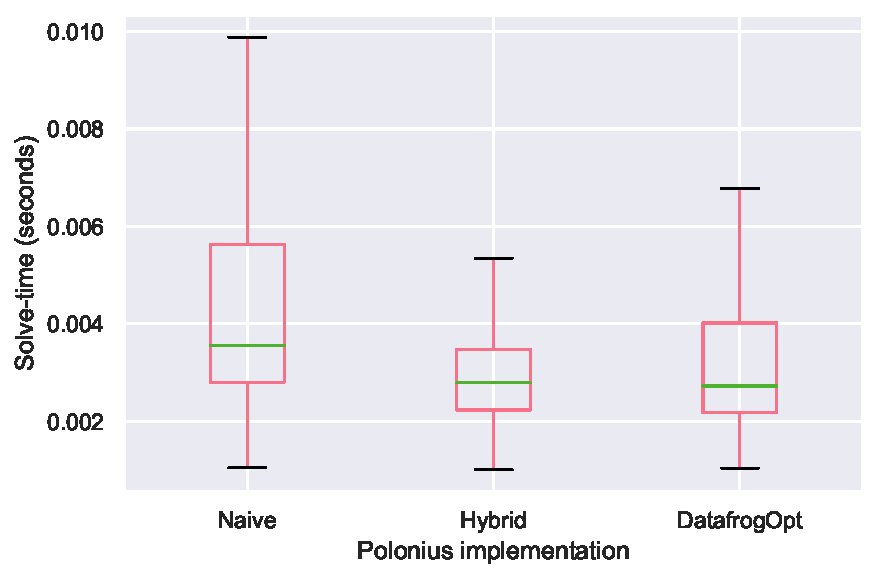
\includegraphics[width=0.9\linewidth]{Graphs/solvetimes_boxplot.pdf}
  \caption[Runtimes Per Function for Three Polonius Variants]{A box plot
    showing the distribution of runtimes per function for three
    implementations of Polonius. As can be seen here, the vast majority execute
    very quickly.}
  \label{fig:solvetimes}
\end{figure}


\begin{figure}
  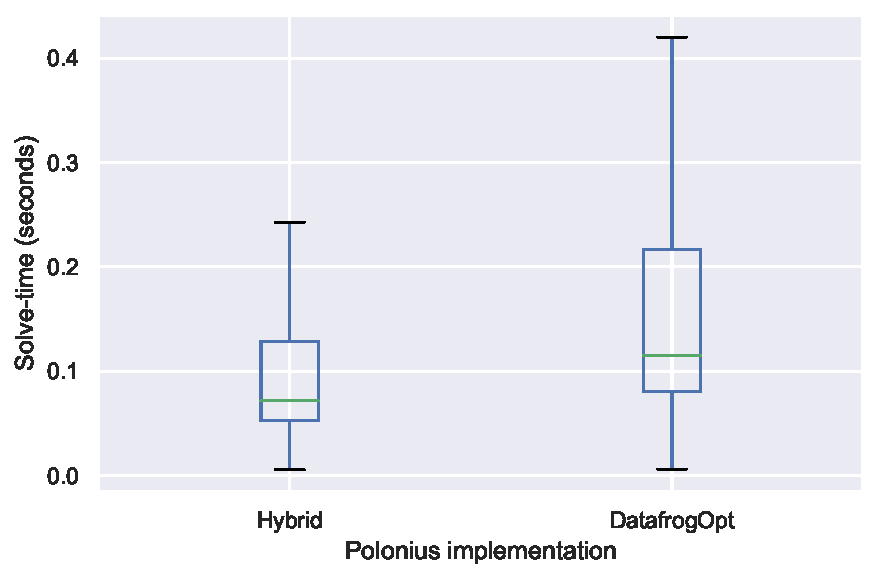
\includegraphics[width=0.9\linewidth]{Graphs/solvetimes_boxplot_over_1s.pdf}
  \caption[Runtimes Per Function for Two Polonius Variants on Longer-Running
  Inputs]{A box plot showing the distribution of runtimes per function for the
    two optimised Polonius implementations on just functions that executed in
    between 1--50s on \textsc{Naive}.}
  \label{fig:solvetimes-long}
\end{figure}

\subsection{Performance}\label{sec:inputs:performance}

In general, all three algorithms finished quickly for almost all functions, with
both of the optimised algorithms already showing improvements in runtimes, as
seen in Figure~\ref{fig:solvetimes}. Apparently, \textsc{Naive} has a wider
spread of runtimes than the others. Additionally, geometric means of the
observed runtimes show improvements from hybridisation
(Figure~\ref{fig:solvetimes-gmean-repo}), though it should be noted that the
algorithm's worst-case of an input that fails both the simple and the full
analysis was left out of the sample as that would have failed compilation,
possibly inflating the results artificially. We can also see clearly that
\textsc{Hybrid} outperforms its fallback flow-sensitive \textsc{DatafrogOpt}
implementation even when excluding smaller inputs~\ref{fig:solvetimes-long}.

\begin{figure}
  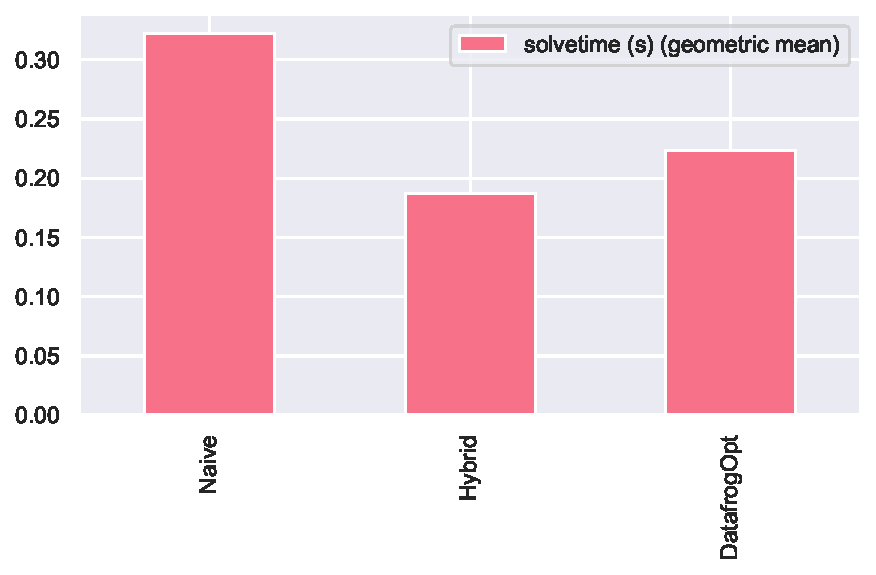
\includegraphics[width=0.5\linewidth]{Graphs/solvetimes_repo_gmean.pdf}
  \caption[Geometric Means of Runtimes Per Repository]{Geometric means of the
    runtimes per repositoriy and implementation.}
  \label{fig:solvetimes-gmean-repo}
\end{figure}


\subsection{Characteristics of Real-World Polonius Input
  Data}\label{sec:inputs:inputs}

\begin{figure}
  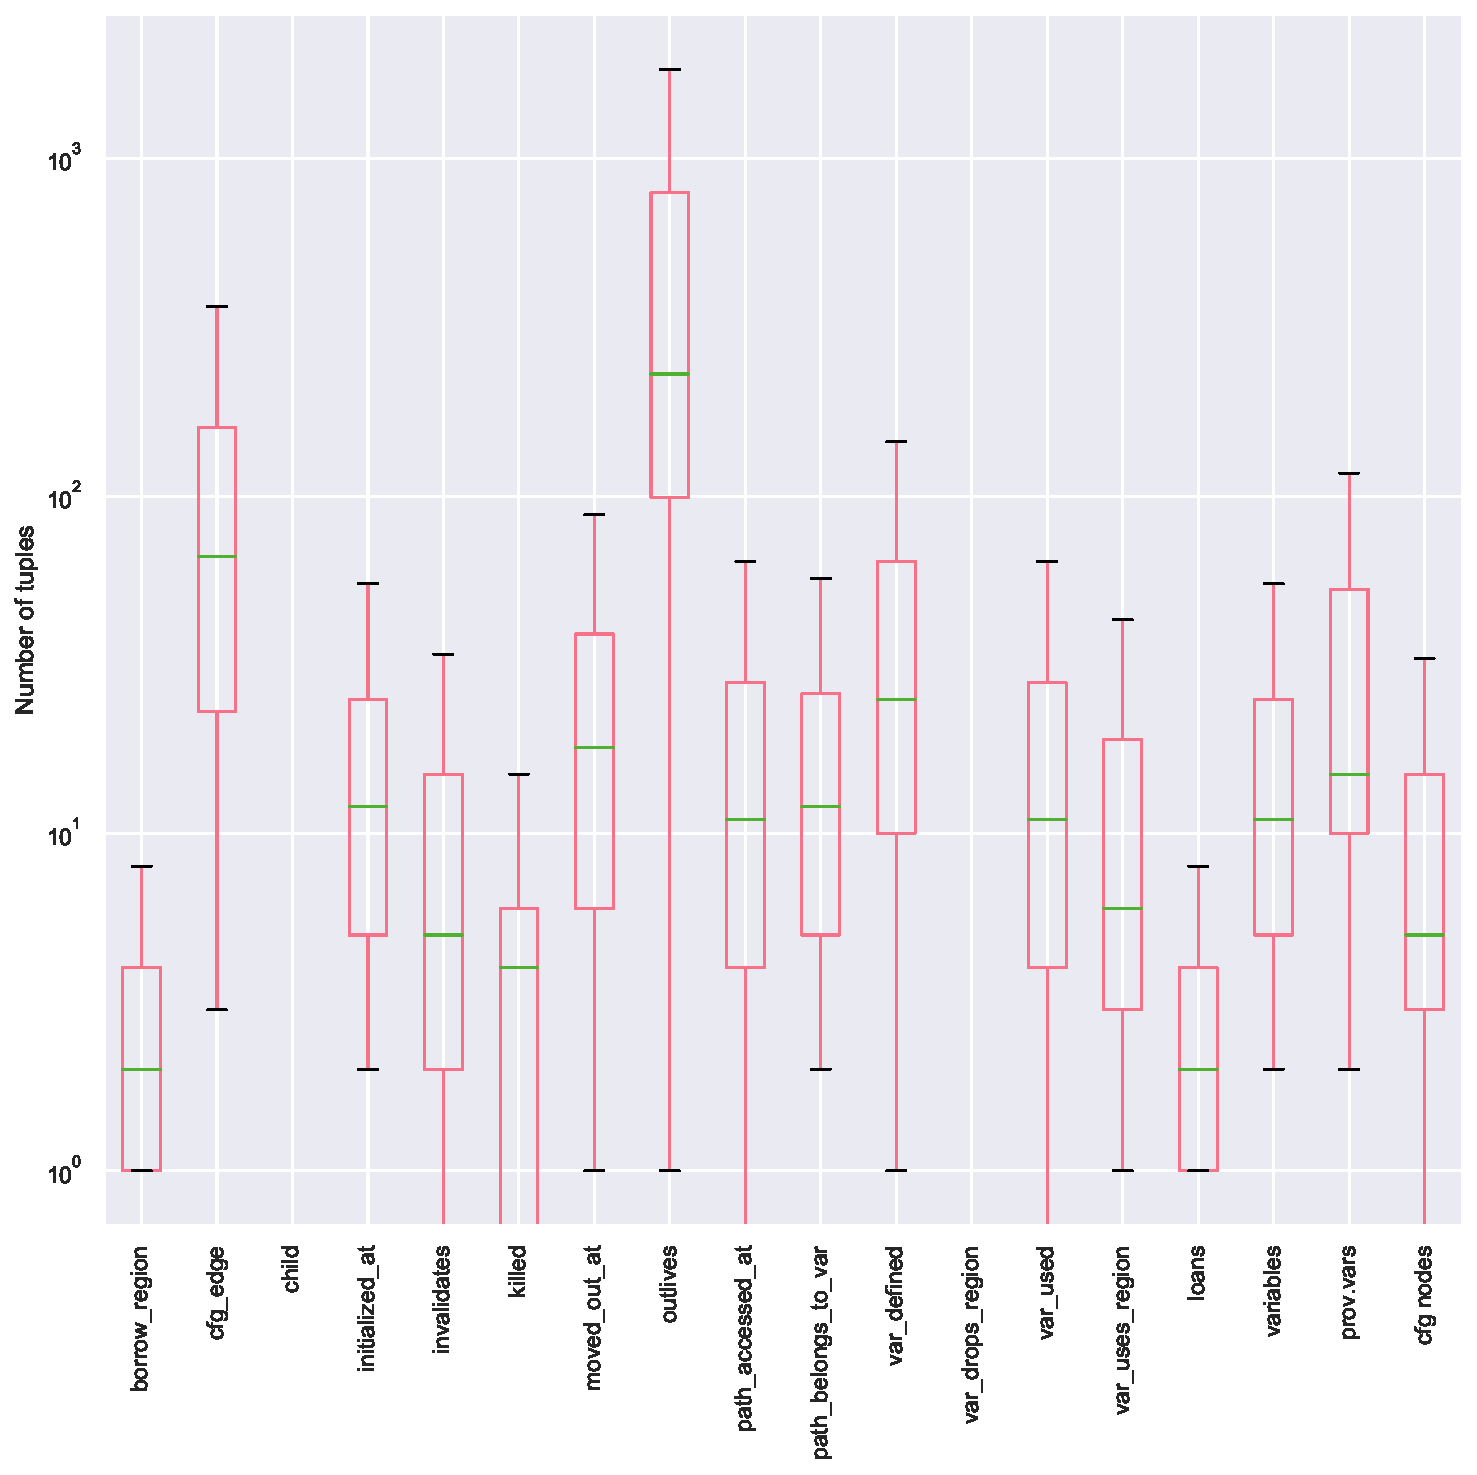
\includegraphics[width=0.9\linewidth]{Graphs/input_sizes_boxplot.pdf}
  \caption[Distribution of Polonius Input Tuple Sizes]{A box plot showing the
    distribution of the various input sizes.}
  \label{fig:input-sizes}
\end{figure}

\begin{figure}
  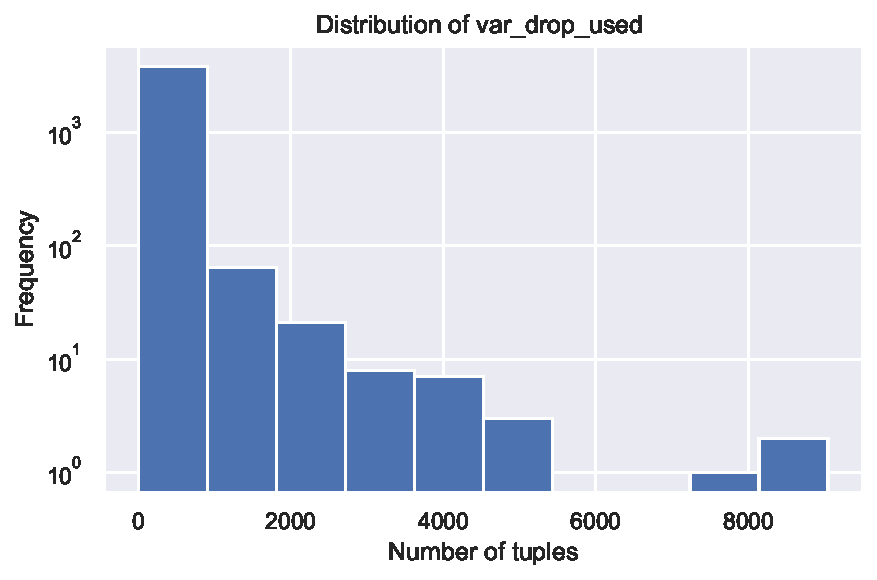
\includegraphics[width=0.5\linewidth]{Graphs/var_drop_used_size_dist.pdf}
  \caption[Distribution of Input Sizes for the \InDatalog{var_drop_used} Fact]{A
    plot showing the distribution of \InDatalog{var_drop_used}.}
  \label{fig:input-var-drop-used}
\end{figure}

A typical Polonius input consists of a small number of tuples for most
relations, as seen in Figure~\ref{fig:input-sizes}. In particular, most
control-flow graphs are small in terms of number of nodes, and most functions
only contain a small number of variables, with an even smaller number of loans.
Drops are particularly rare, with circa~70\% of all studied functions having
no (potential) drop-uses at all (0 median, 7.6 mean), and only very few
loans (2~median, 5~mean). This can also be seen in
Figure~\ref{fig:input-var-drop-used} showing the distribution of number of
(potential) drop-uses per function. In practice, this means that users generally
do not override the built-in deallocators, do not explicitly deallocate their
variables. The low number of loans also means that functions in general do not
use complicated reference-sharing, typically only manipulating a few references.

This points towards a need to have a low starting overhead for Polonius, as
much of its analysis would have to be performed on very small inputs, where the
runtime would be dominated by a high constant setup time.

However, repositories can be assumed to be typically compiled all at once.
Therefore, it is also interesting to say something about the maximum input size
per repository, under the assumption that few large functions would dominate the
runtime for that repository. After collecting the maximum values per repository,
the median number of loans was~24, and the median number of potential drop-uses
was~45 (regular uses was, for comparison, 177).

We attempted to perform a principal-component analysis (PCA) of the input data
in order to visually identify possible clusterings of types of inputs, but the
results were unusable as the inputs had no visually discernible patterns in
neither 2 nor 3 dimensions, suggesting that most inputs are in some sense
typical, or that PCA is ineffective here.

\subsection{How Inputs Affect Runtime}\label{sec:inputs:correlation}
\begin{figure}
  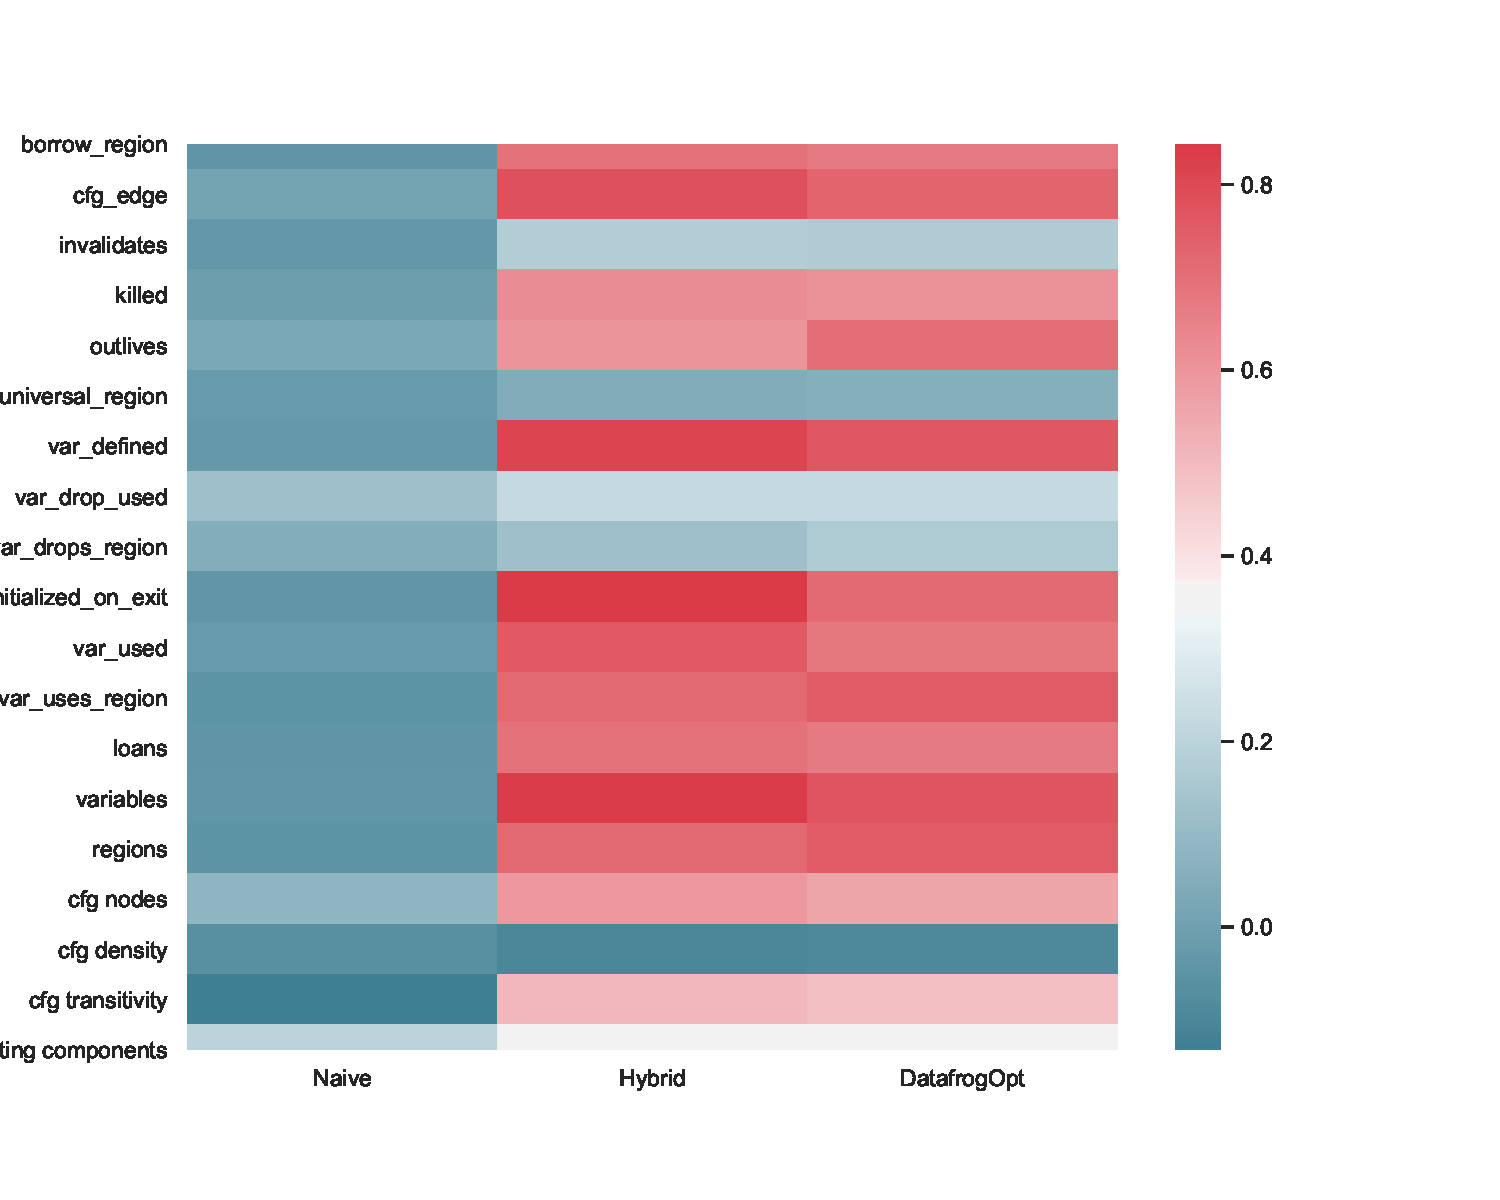
\includegraphics[width=0.9\linewidth]{Graphs/corr_heatmap.pdf}
  \caption[Heatmap of Input Sizes Affecting Runtime]{Heatmap of
    Pearson~correlations between various input size metrics and runtimes for
    all three Polonius implementations, suggesting in particular that variable
    uses, number of variables, and the number of provenance variables heavily
    affect runtime.}
  \label{fig:corr-heatmap}
\end{figure}
A heatmap of the (Pearson) correlation between input size and runtime for the
various variants on long-running jobs (as previously defined to be jobs taking
at least 1s and no more than 50s to run under \textsc{Naive}) can be seen in
Figure~\ref{fig:corr-heatmap} and Table~\ref{tab:correlations}, while a scatter
plot of the results with a linear regression for some interesting pairs of
inputs can be seen in Figure~\ref{fig:input-scatter}.

\begin{table}[ht]
  \begin{tabular}{lrrr}
\toprule
{} &     Naive &    Hybrid &  DatafrogOpt \\
\midrule
var\_used            &  0.363947 &  0.531098 &     0.531099 \\
path\_accessed\_at    &  0.349286 &  0.497498 &     0.498295 \\
variables           &  0.304380 &  0.418331 &     0.423401 \\
initialized\_at      &  0.309505 &  0.403256 &     0.407881 \\
path\_belongs\_to\_var &  0.298802 &  0.398564 &     0.403784 \\
var\_defined         &  0.279185 &  0.340064 &     0.348787 \\
cfg\_edge            &  0.296521 &  0.313906 &     0.322021 \\
moved\_out\_at        &  0.286129 &  0.295944 &     0.302707 \\
prov.vars           &  0.193118 &  0.222522 &     0.239422 \\
var\_uses\_region     &  0.175650 &  0.195924 &     0.212868 \\
cfg nodes           &  0.279858 &  0.193068 &     0.200334 \\
child               &  0.270583 &  0.195513 &     0.168010 \\
loans               &  0.137711 &  0.133432 &     0.151154 \\
borrow\_region       &  0.137711 &  0.133432 &     0.151154 \\
killed              &  0.080521 &  0.101943 &     0.102579 \\
invalidates         &  0.044914 &  0.082414 &     0.084853 \\
outlives            &  0.206378 &  0.062142 &     0.082695 \\
var\_drop\_used       &  0.195021 &  0.031959 &     0.043753 \\
var\_drops\_region    &  0.135435 &  0.013908 &     0.023246 \\
\bottomrule
\end{tabular}

  \caption[Pearson Correlations Between Sizes of Inputs and Runtime]{Pearson
    correlations between size of inputs and the runtime of \textsc{Naive},
    \textsc{Hybrid}, and \textsc{DatafrogOpt} respectively, from high
    correlation to \textsc{DatafrogOpt} runtime to low.}
  \label{tab:correlations}
\end{table}%

It is clear here that inputs affecting all parts of the computation have a
larger influence, notably variable uses, number of variables, and the number of
provenance variables. In particular, input sizes affecting the liveness
computation time affects \textsc{Hybrid}, which should be no surprise as it does
that computation twice. The same goes for the number of provenance variables,
which figure in the second two parts of the analysis. Another conclusion from
Table~\ref{tab:correlations} is that the number of nodes of the CFG has a lower
impact on runtime than its number of edges, reflecting that complex CFGs with
many branchings take more time to compute than linear ones.

Both results suggest only a weak linear relation between input sizes and
and the runtime with \textsc{Naive}, while a clearer relation can be
found between \textsc{DatafrogOpt} and input sizes respectively. \textsc{Naive},
on the other hand, does not show similarly clear correlations between runtime
and input sizes of any kind (Table~\ref{tab:correlations}).

\begin{figure}
  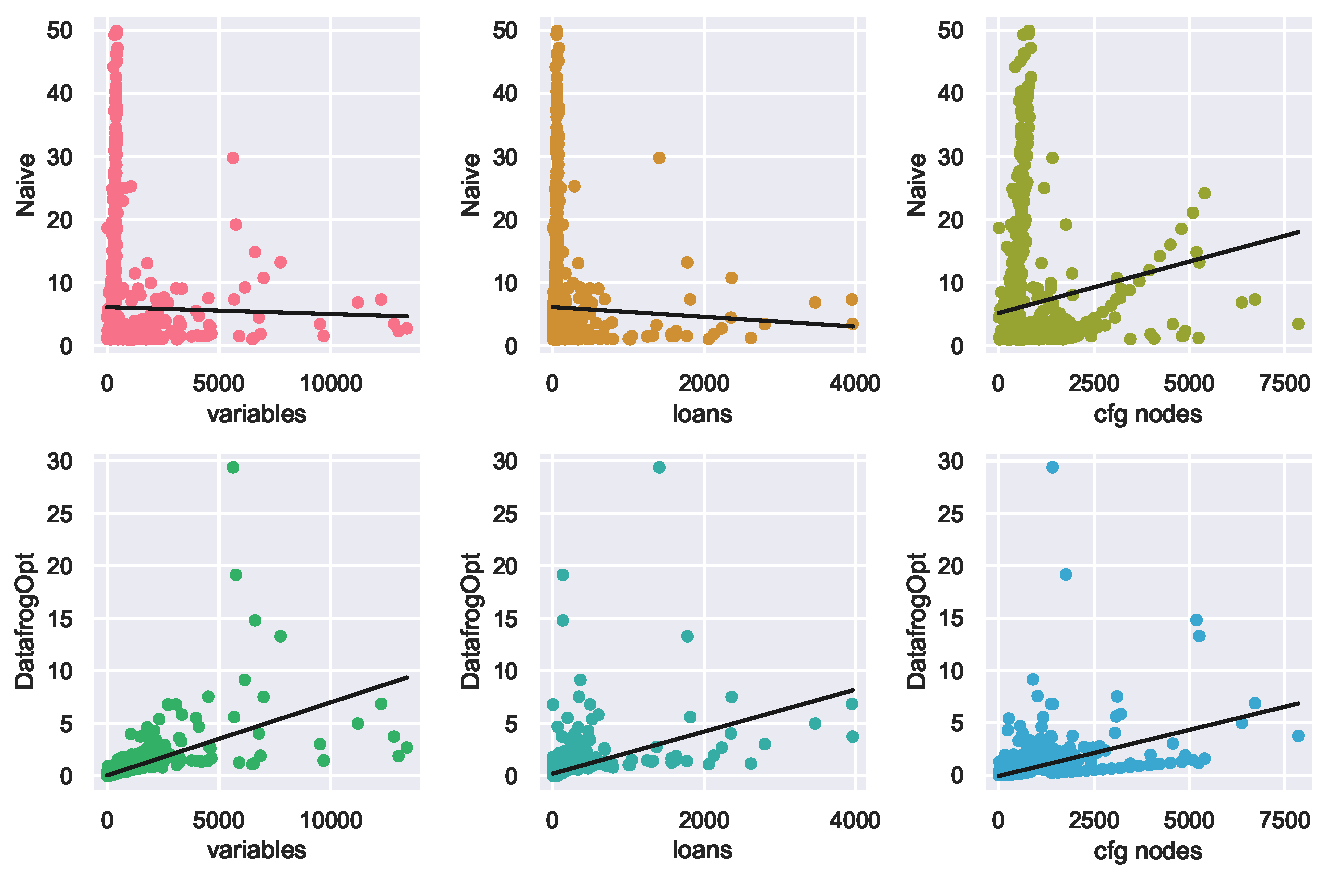
\includegraphics[width=0.9\linewidth]{Graphs/corr_scatter.pdf}
  \caption[Scatter Plot of Runtimes On Two Polonius Variants vs. nr. of CFG
  Edges and Variables]{Scatter plot of runtimes under the naive and optimised
    algorithms compared to variables and CFG edge count after having pruned
    extreme values (runtimes below 1~s or above 13~minutes). Y~axis is runtime
    in seconds.}
  \label{fig:input-scatter}
\end{figure}

\chapter{Conclusions and Future Work}\label{cha:conclusions}
\epigraph{To sleep: perchance to dream: ay, there's the rub;\\
  For in that sleep of death what dreams may come}%
{\textit{Hamlet}, Act-III, Scene-I}

Before Polonius can replace NLL as the Rust borrow checker, it would need
considerable performance improvements in both its fact generation process as
well as the solving itself. In its current condition, the fact generation code,
in particular, performs multiple walks across the CFG, needlessly increasing
runtime. Additionally, many of the inputs are computed unnecessarily, and, for
example, the CFG could be compressed for some cases.

Returning to the analysis of Section~\ref{sec:field-study-borrow}, we can see
from the performance of even the current naive \textsc{Hybrid} implementation,
which first performs a non-flow sensitive analysis and then falls back to the
full Polonius analysis, outperforms both the optimised analysis alone and
\textsc{Naive}. We can also see that inputs without any loans at all are common,
and in those cases the analysis can typically terminate before performing any
analysis at all. Finally, \textsc{Naive} could be improved in two ways. First,
in the current implementation initialisation and liveness analysis is performed
twice for purely architectural reasons. A better implementation would calculate
them once and re-use the results. Second, the current analysis does not use the
errors from the flow-insensitive analysis when it falls back to the full
flow-sensitive Polonius. Recycling the errors from the first analysis could in
many cases reduce the search space for Polonius significantly, as any other
error has already been ruled out in the simpler analysis.

Finally, Datafrog itself could be optimised, including using faster vector
instructions or parallelisation techniques. Additionally, several of the input
relations used in Polonius are only used to exclude values, and never used to
propagate them. This suggests it would be possible to use more compact data
structures for representing them, such as Bloom filters.

In this report, we have described a first implementation of the Rust borrow
check in Datalog. We have shown how partial initialisation tracking was used
along with variable-use and definition data to determine live references, which
were then used to detect which potential loan violations happening in the code
would actually be of a live reference, therefore causing an error.

Building on top of this, we then analysed Rust code from  ca~12~000 popular Git
repositories to determine what a characteristic Polonius input would look like.
The study found that relatively few functions use any references at all,
suggesting that the borrow check should be able to terminate early in a
significant number of cases. On the same note, we also found that foregoing the
full flow-sensitive analysis and falling back on a simpler analysis, even
naively, in many cases improves performance significantly. Finally, the study
concluded that the number of transitions in the control-flow graph and the
number of variables both would be good proxies for the difficulty of solving an
input in Polonius, in terms of run-time.

Left to do in Polonius before it is feature-complete is integrating it with the
Rust type checker for higher-order kinds, finishing the full initialisation
tracking, and extending the analysis to also include illegal subset constraints
on reference type provenance variables. Finally, we also briefly discussed a
recently discovered shortcoming believed to exist in both Polonius and the Oxide
formulation~\cite{weiss_oxide:_2019}, related to provenance variable imprecision
in the analysis causing spurious errors. This issue is currently under
investigation, and addressing it would likely impact the performance of
Polonius, though possibly in a positive direction as a less precise formulation
would potentially (in some cases) produce fewer tuples to propagate during
analysis.

\begin{figure}
  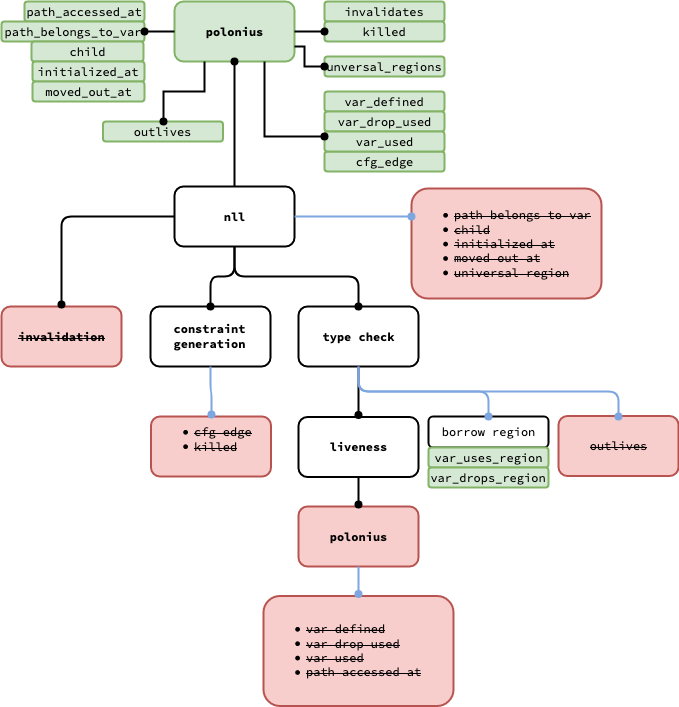
\includegraphics[width=\linewidth]{Graphs/polonius-refactor}
  \caption[Suggested Refactoring for the Polonius Fact Generation in Rust]{A
    suggestion for how the Polonius fact generation in Rust can be reorganised.
    Green boxes show inputs, black boxes Rust modules, and red modules (re)moved
    components. Note that boxes are grouped together according to the inputs
    necessary for producing them.}
  \label{fig:fact-refactor}
\end{figure}

Finally, there is a need to refactor both Polonius itself (whose interface is
outside the scope of this thesis), and the fact generation code of
Figure~\ref{fig:fact-module-hierarchy}. Such a refactoring could even reduce the
number of iterations over the MIR during input generation, decreasing the
runtime of that part of the code. A proposal for how the fact-generation code
could be reorganised is shown in Figure~\ref{fig:fact-refactor}. The key idea is
to divide the fact generation code according to where in the compilation process
it takes is inputs, such that only the parts needing access to the internal
parts of the type-checker are executed during type-checking. This grouping of
code according to the data it operates on also means that costly operations,
notably CFG iteration, can be performed all at once.

\Urlmuskip=0mu plus 15mu\relax
%\backmatter
\printbibliography[heading=bibintoc]
\end{document}